\chapter{Fourier-Theorie f"ur die Kugeloberfl"ache
\label{chapter:kugel}}
\lhead{Fourier f"ur die Kugeloberfl"ache}
\begin{refsection}
\chapterauthor{Thomas Gujer und Christoph Schmitz-Dr"ager}

\section{Einleitung}
\rhead{Einleitung}
In diesem Kapitel m"ochten wir veranschaulichen, dass die Ph"anomene, 
der klassischen Fourier-Theorie, auch auf der Kugeloberfl"ache zu 
sehen sind.
Zur Visualisierung vergleichen wir jeweils ein Rechtecksignal mit 
dem Analogon auf der Kugeloberfl"ache.

\section{Funktionen auf der Kugeloberfl"ache}
\rhead{Funktionen auf der Kugeloberfl"ache}
Im Gegensatz zu den Funktionen, die mittels klassischer 
Fourier-Theorie analysiert werden, h"angen Funktionen auf der 
Kugeloberfl"ache von drei Variablen ab. 
Da der Funktionswert aber nicht in einer weiteren Dimension 
dargestellt werden kann, muss man auf andere Mittel zur"uckgreifen. 
Das bedeutet, dass die drei Variablen die geometrischen Position
auf der Kugeloberfl"ache bestimmen und dass der Funktionswert 
mittels Farbcodierung dargestellt wird. 
Dies entspricht der selben Darstellung, die z.B. auch f"ur die 
Temperatur auf der Erdoberfl"ache verwendet wird. In diesem Fall 
darf man die Form der Erde auch nicht beeinflussen um die Temperatur 
darzustellen.
\subsection{Kugelkoordinaten}
\begin{figure}%Bild Koordinaten der Kugel
\centering
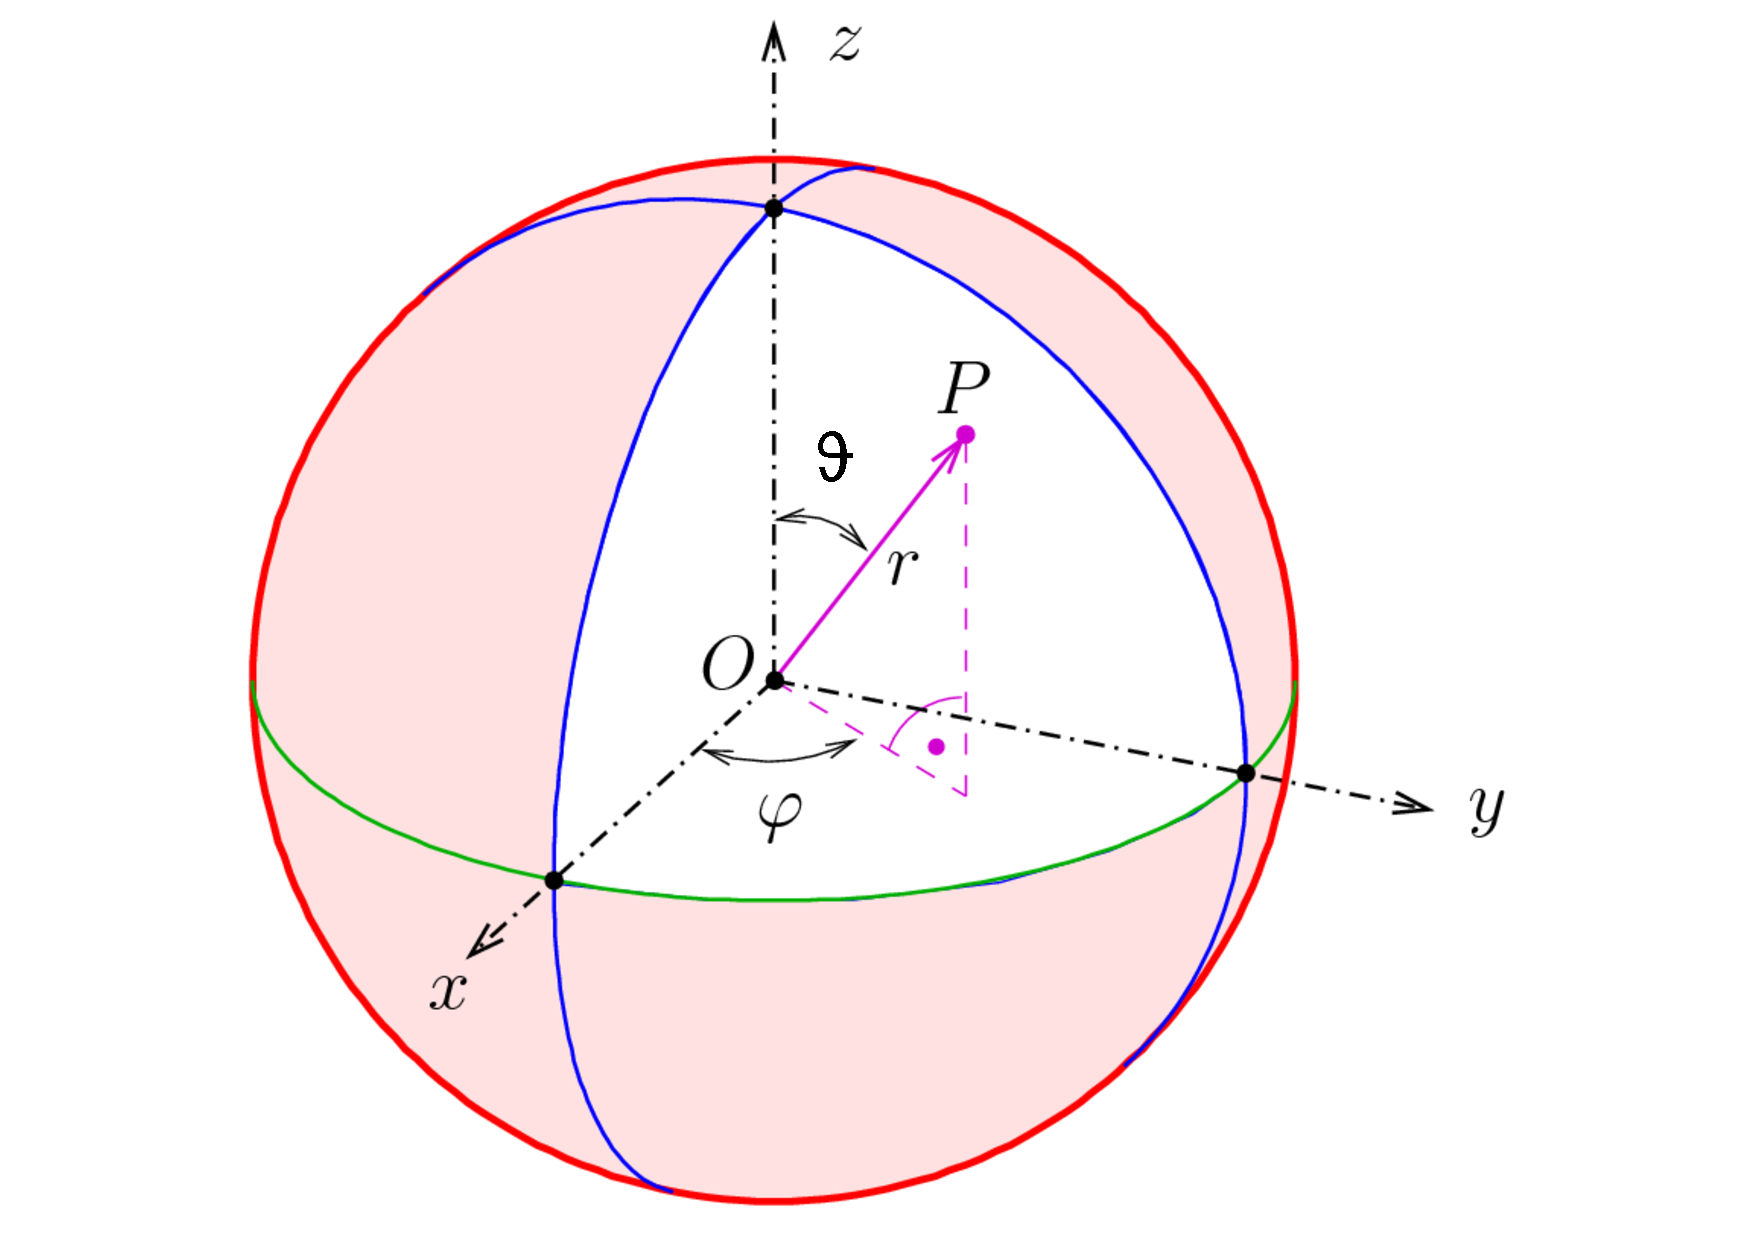
\includegraphics[width=0.7\textwidth]{kugel/Kugelkoord.pdf}
\caption{Koordinaten der Kugel
\label{skript:Koordinaten der Kugel}}
\end{figure}

Abbildung \ref{skript:Koordinaten der Kugel} 
zeigt wie eine Position auf der Kugeloberfl"ache in
Kugel-Koordinaten definiert ist. 
Da wir uns in diesem Kapitel aber nur auf der Oberfl"ache der 
Einheitskugel bewegen wird der Radius r konstant auf 1 gesetzt. 
Durch Variation des Winkels $\vartheta$ ver"andern wir die 
geographische Breite. 
Mit dem Winkel $\varphi$ variieren wir die geographische 
L"ange. 
Dadurch l"asst sich jede Position auf der Kugeloberfl"ache definieren. 
Zum Umrechnen ins kartesische Koordinatensystem verwenden wir die 
Formeln:
\[
\left.\begin{aligned}
x& = \sin\vartheta \cdot \cos\varphi\\
y& = \sin\vartheta \cdot \sin\varphi\\
z& = \cdot \cos\vartheta\\      
\end{aligned}
\right\}
\qquad (0 \leq \vartheta \leq \pi \wedge {-\pi} \leq \varphi \leq \pi)
\]

\subsection{Rechteckfunktionen}
\begin{figure}%Funktion auf Rechteckoberfläche 
\centering
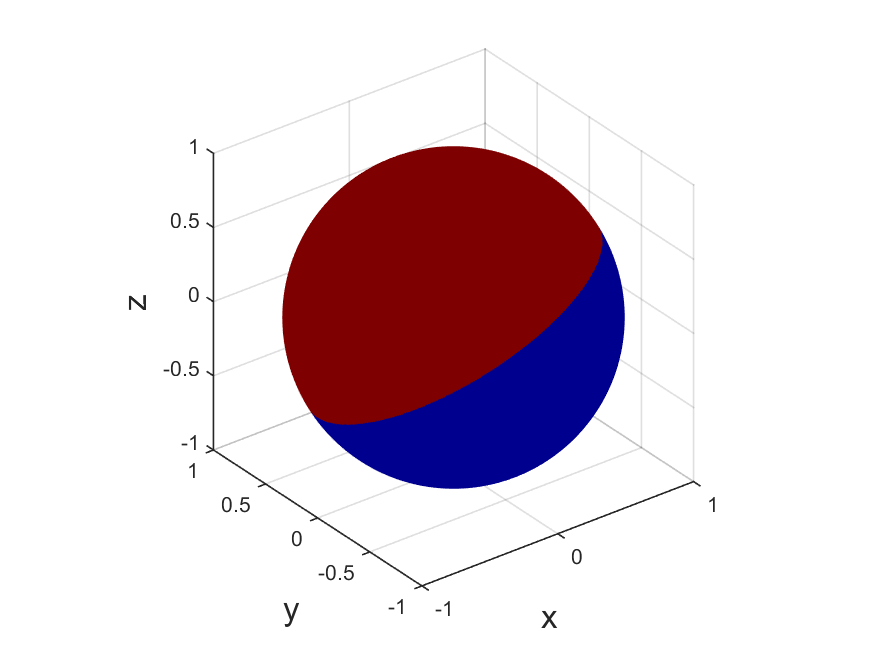
\includegraphics[width=0.5\textwidth]{kugel/Funktion.pdf}
\caption{Funktion auf der Kugeloberfl"ache
\label{skript:Funktion auf Kugeloberfl"ache}}
\end{figure}
In unseren Beispielen wird die $2\pi$-periodische Rechteckfunktion
mit den Funktionswerten 0 und 1 definiert. 
Die Funktion auf der Kugeloberfl"ache wird analog 
mit denselben Funktionswerten definiert. 
Dabei wird einem kreisf"ormigen Abschnitt auf der Kugeloberfl"ache 
der Wert 1 zugewiesen und dem Rest der Kugeloberfl"ache der 
Funktionswert 0. 

Eine $2\pi$-periodische Rechteckfunktion ist folgendermassen definiert:
\begin{equation}
f(x) =
\begin{cases}
1 & \text{f"ur } u+2\pi k \leq x \leq v + 2\pi k , k \in \mathbb{Z}
\\
0 & \text{sonst } 
\end{cases}
\label{skript:Rechteckfunktion Formel}
\end{equation}
Die Parameter $u$ und $r$ mit $0 \leq u \leq v \leq 2\pi$ markieren
die aufsteigende, respektive die fallende Flanke. 

Das Analogon auf der Kugeloberfl"ache bauen wir wie folgt auf:
\begin{enumerate}
\item Wir definieren einen Vektor $\vec{c}$ mit den Kugel-Koordinaten
$\vartheta_c$ und $\varphi_c$.
Der Startpunkt dieses Vektors liegt im Zentrum der Kugel und der
Endpunkt auf der Kugeloberfl"ache:

\begin{equation}
\vec{c} = 
\begin{pmatrix}
{\sin\vartheta_c \cdot \cos\varphi_c}\\
{\sin\vartheta_c \cdot \sin\varphi_c}\\
{\cos\vartheta_c}
\end{pmatrix}
\label{skript:Vektor c Formel}
\end{equation}
$$
\vartheta_x \in [ 0, \pi ] \wedge \varphi_y \in [ -\pi, \pi ]
$$

\item Des Weiteren definieren die Vektoren $\vec{r} (\vartheta, \varphi)$.
Sie haben, wie der Vektor $\vec{c}$ die Startpunkte im Zentrum der 
Kugel und die Endpunkte auf der Kugeloberfl"ache. 
Im Gegensatz zu Vektor $\vec{c}$ werden jedoch die Vektoren  
$\vec{r}$ der Vektorschar $r$ mit den Kugelkoordinaten
$\vartheta$ und $\varphi$ definiert.
\[
\vec{r} (\vartheta, \varphi) = 
\begin{pmatrix}
{\sin\vartheta \cdot \cos\varphi}\\
{\sin\vartheta \cdot \sin\varphi}\\
{\cos\vartheta}
\end{pmatrix}
\quad
0 \leq \vartheta \leq \wedge -\pi \leq \varphi \leq \pi
\]

\item Als letztes berechnen wir die Skalarprodukte des Vektors $\vec{c}$
und den Vektoren $\vec{r} (\vartheta, \varphi)$.
Dadurch erh"alt man den Kosinus des Zwischenwinkels des Vektors $\vec{c}$
und dem jeweiligen Vektor $\vec{r} (\vartheta, \varphi)$.
Mit dem Parameter $w$ legt man letztlich fest wie gross der 
Kreisabschnitt werden soll, dem der Wert eins zugewiesen wird.
\begin{equation}
f(\vartheta, \varphi) =\begin{cases}
1 & \text{wenn } \vec{c} \cdot \vec{r} (\vartheta, \varphi) \geq w\\
0 & \text{sonst}
\end{cases}
\label{skript:Kugelfunktion Formel}
\end{equation}
\end{enumerate}
\section{Fourier-Theorie}
\rhead{Fourier-Theorie}
In diesem Abschnitt m"ochten wir die Theorie der Fourier-Theorie
auf der Kugeloberfl"ache vermitteln. 
Zum einfacheren Verst"andnis wird immer zuerst die Formel der 
klassischen Fourier-Theorie aufgezeigt, bevor die Formel der 
Fourier-Theorie auf der Kugeloberfl"ache dargestellt wird.

\subsection{Kugelfl"achenfunktionen}
Bei der klassischen Fourier-Theorie sind die Analoga zu den Sinus- 
und Kosinus-Funktionen die Kugelfl"achenfunktionen. 
Mittels dieser Kugelfl"achenfunktionen $Y_{lm}$ und $Z_{lm}$ 
bildet man ein orthogonales System von Funktionen. 
Die Kugelfl"achenfunktionen sind wie folgt definiert:
\begin{align*}
Y_{lm}(\vartheta, \varphi)& = P_{lm} \cdot (\cos \varphi) \cdot \cos(m \cdot \varphi)
\\
Z_{lm}(\vartheta, \varphi)& = P_{lm} \cdot (\cos \varphi) \cdot \sin(m \cdot \varphi)
\end{align*}
Bei $P_{lm}$ handelt es sich um das in Kapitel \ref{skript:legendreansatz} 
hergeleitete Legendre-Polynom. 
Mit $l$ wird der Grad des Legendre-Polynoms angegeben und f"ur $m$
gilt die Bedingung $0 \leq m \leq l$.  
In Abbildung \ref{skript:ylm l=5 m=0} bis \ref{skript:zlm l=5 m=5} sieht man die verschiedenen 
Kugelfl"achenfunktionen vom Grad $l = 5$.

\begin{figure}
\begin{minipage}[hbt]{0.4\textwidth}
\centering
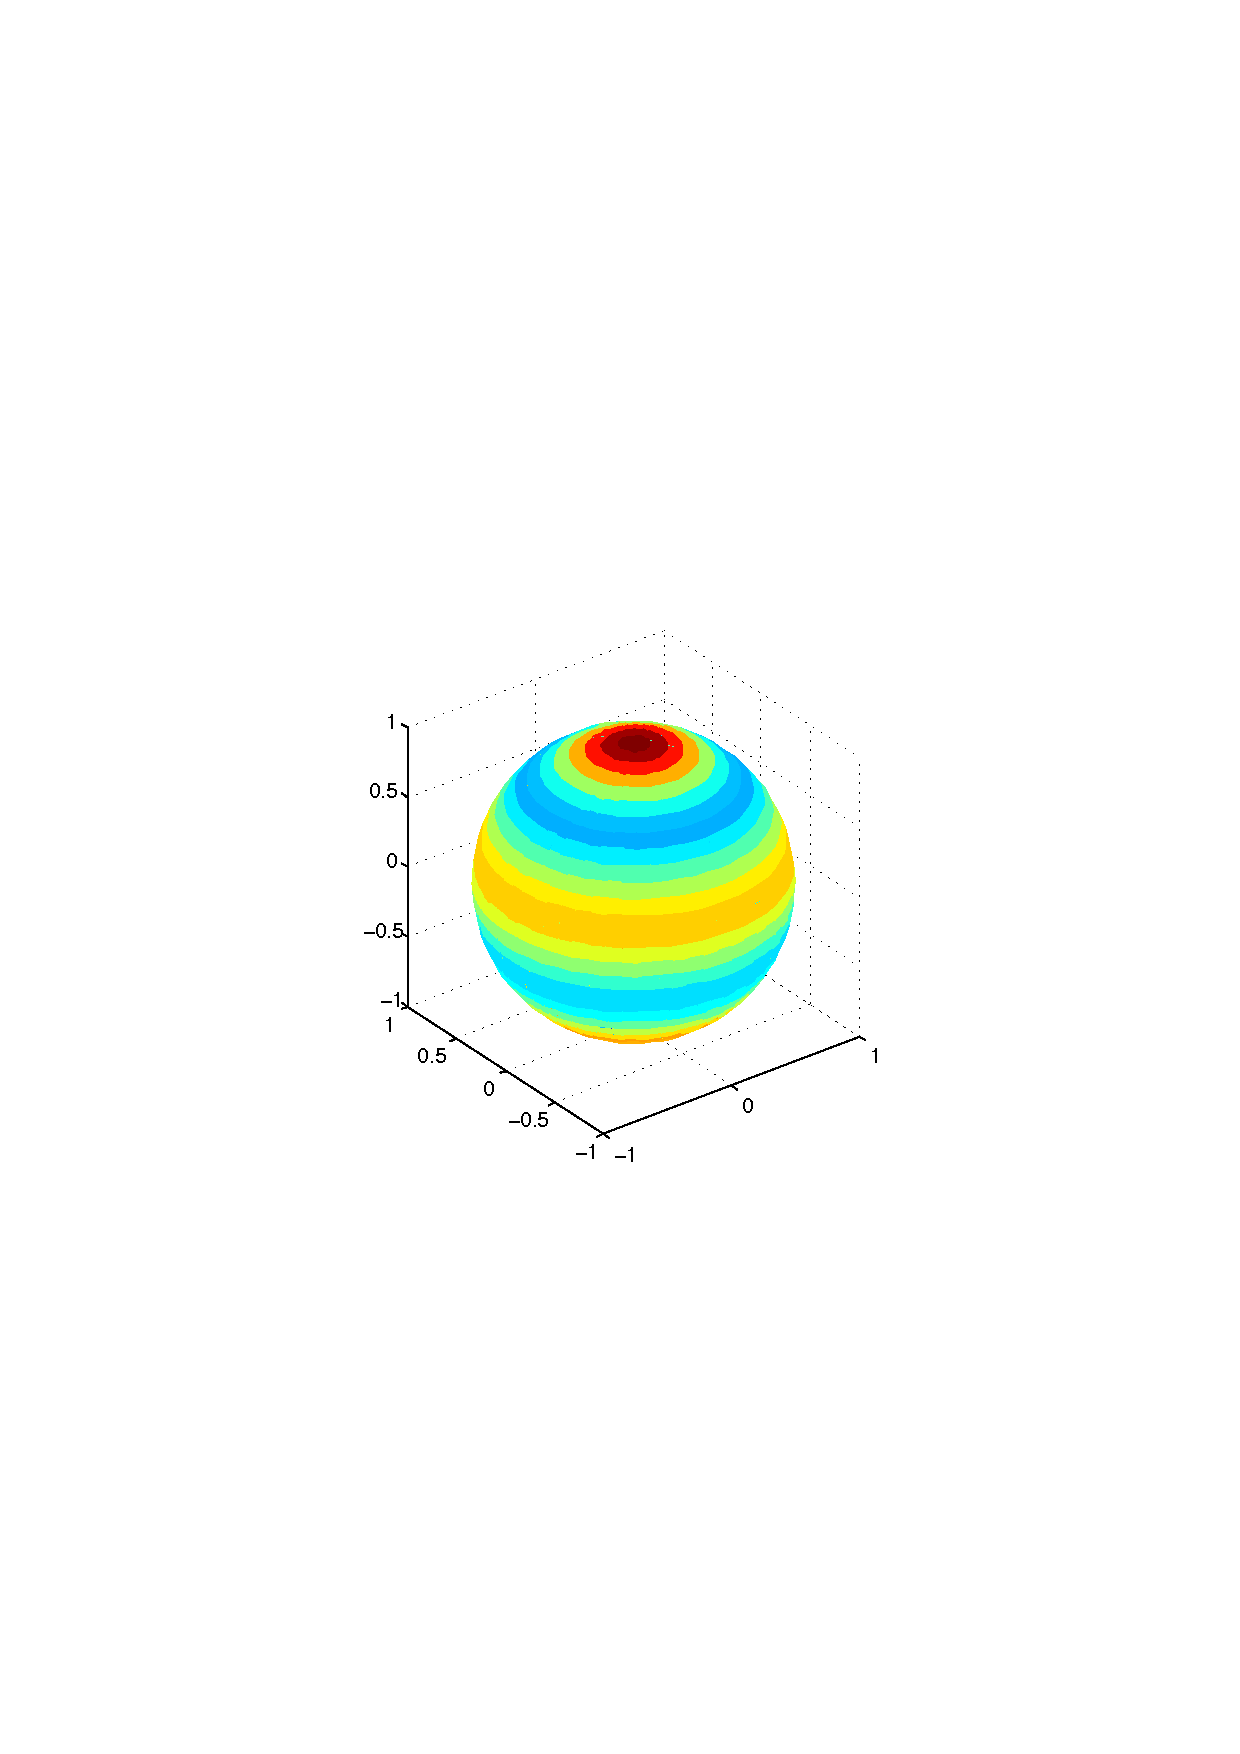
\includegraphics[width=1\textwidth]{kugel/ylm/a_5_0.pdf}
\caption{$Y_{lm}$ mit $l=5$, $m=0$}
\label{skript:ylm l=5 m=0}
\end{minipage}
\hfill
\begin{minipage}[hbt]{0.4\textwidth}
\centering
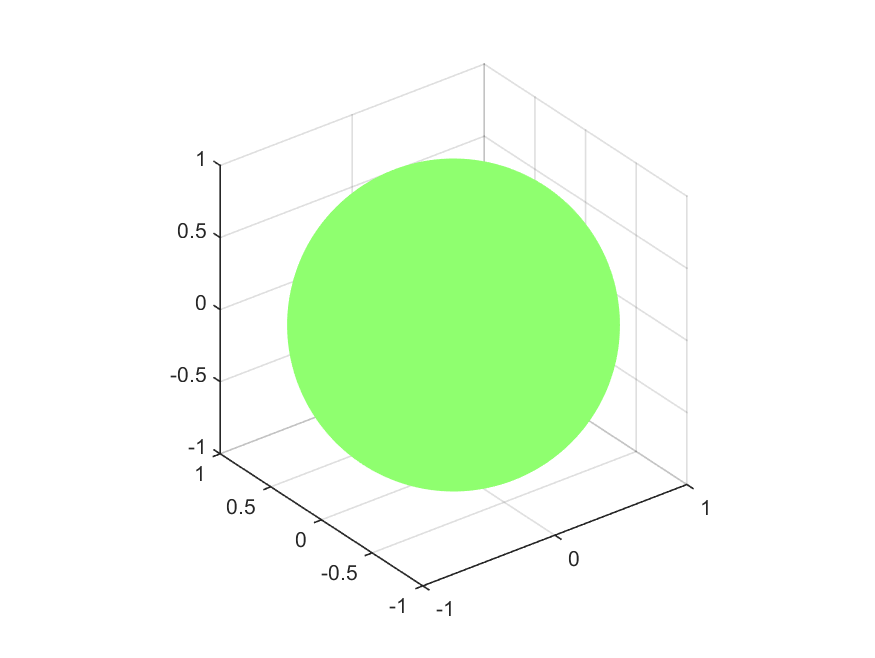
\includegraphics[width=1\textwidth]{kugel/ylm/b_5_0.pdf}
\caption{$Z_{lm}$ mit $l=5$, $m=0$}
\label{skript:zlm l=5 m=0}
\end{minipage}
\begin{minipage}[hbt]{0.4\textwidth}
\centering
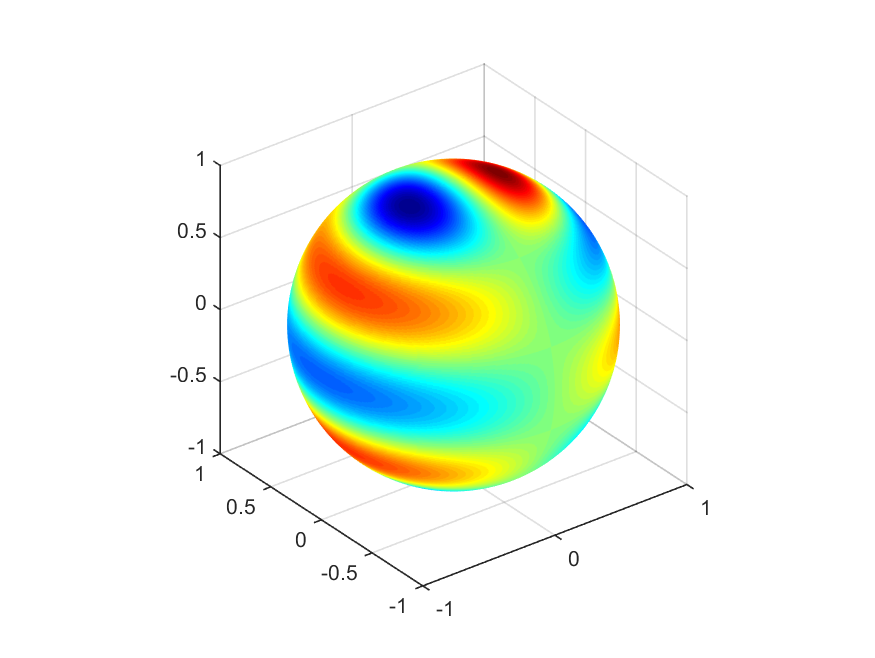
\includegraphics[width=1\textwidth]{kugel/ylm/a_5_1.pdf}
\caption{$Y_{lm}$ mit $l=5$, $m=1$}
\label{skript:ylm l=5 m=1}
\end{minipage}
\hfill
\begin{minipage}[hbt]{0.4\textwidth}
\centering
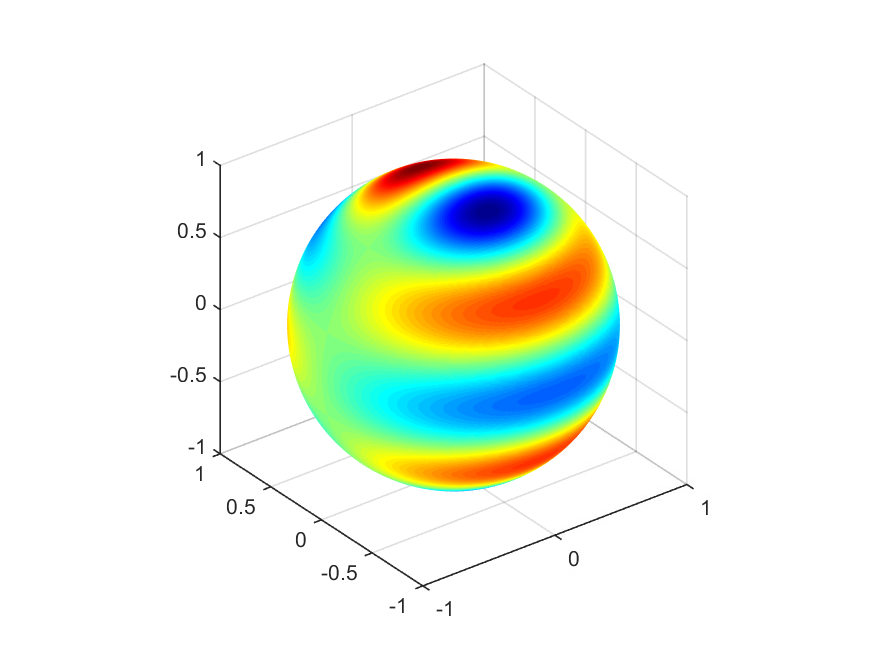
\includegraphics[width=1\textwidth]{kugel/ylm/b_5_1.pdf}
\caption{$Z_{lm}$ mit $l=5$, $m=1$}
\label{skript:zlm l=5 m=1}
\end{minipage}
\begin{minipage}[hbt]{0.4\textwidth}
\centering
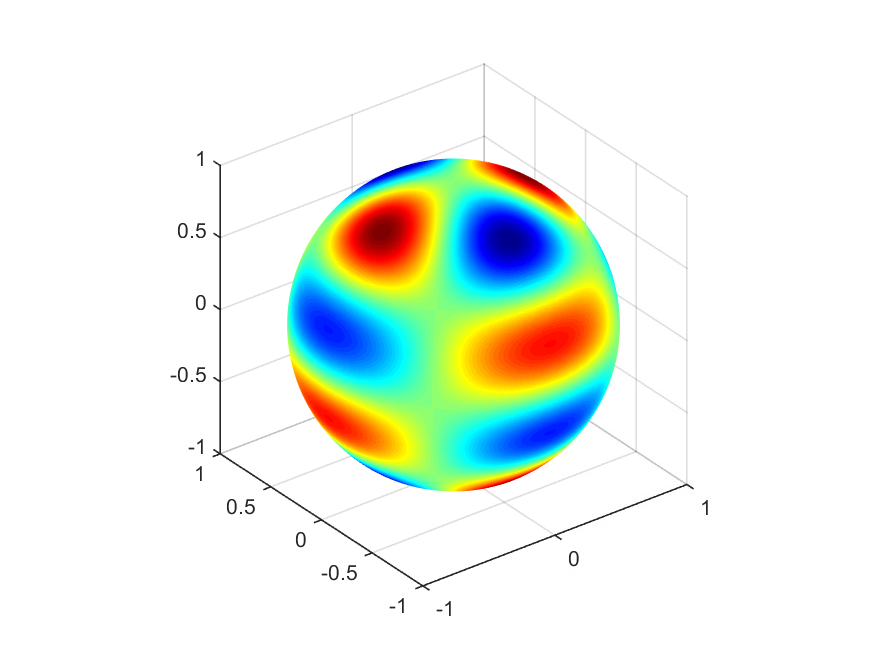
\includegraphics[width=1\textwidth]{kugel/ylm/a_5_2.pdf}
\caption{$Y_{lm}$ mit $l=5$, $m=2$}
\label{skript:ylm l=5 m=2}
\end{minipage}
\hfill
\begin{minipage}[hbt]{0.4\textwidth}
\centering
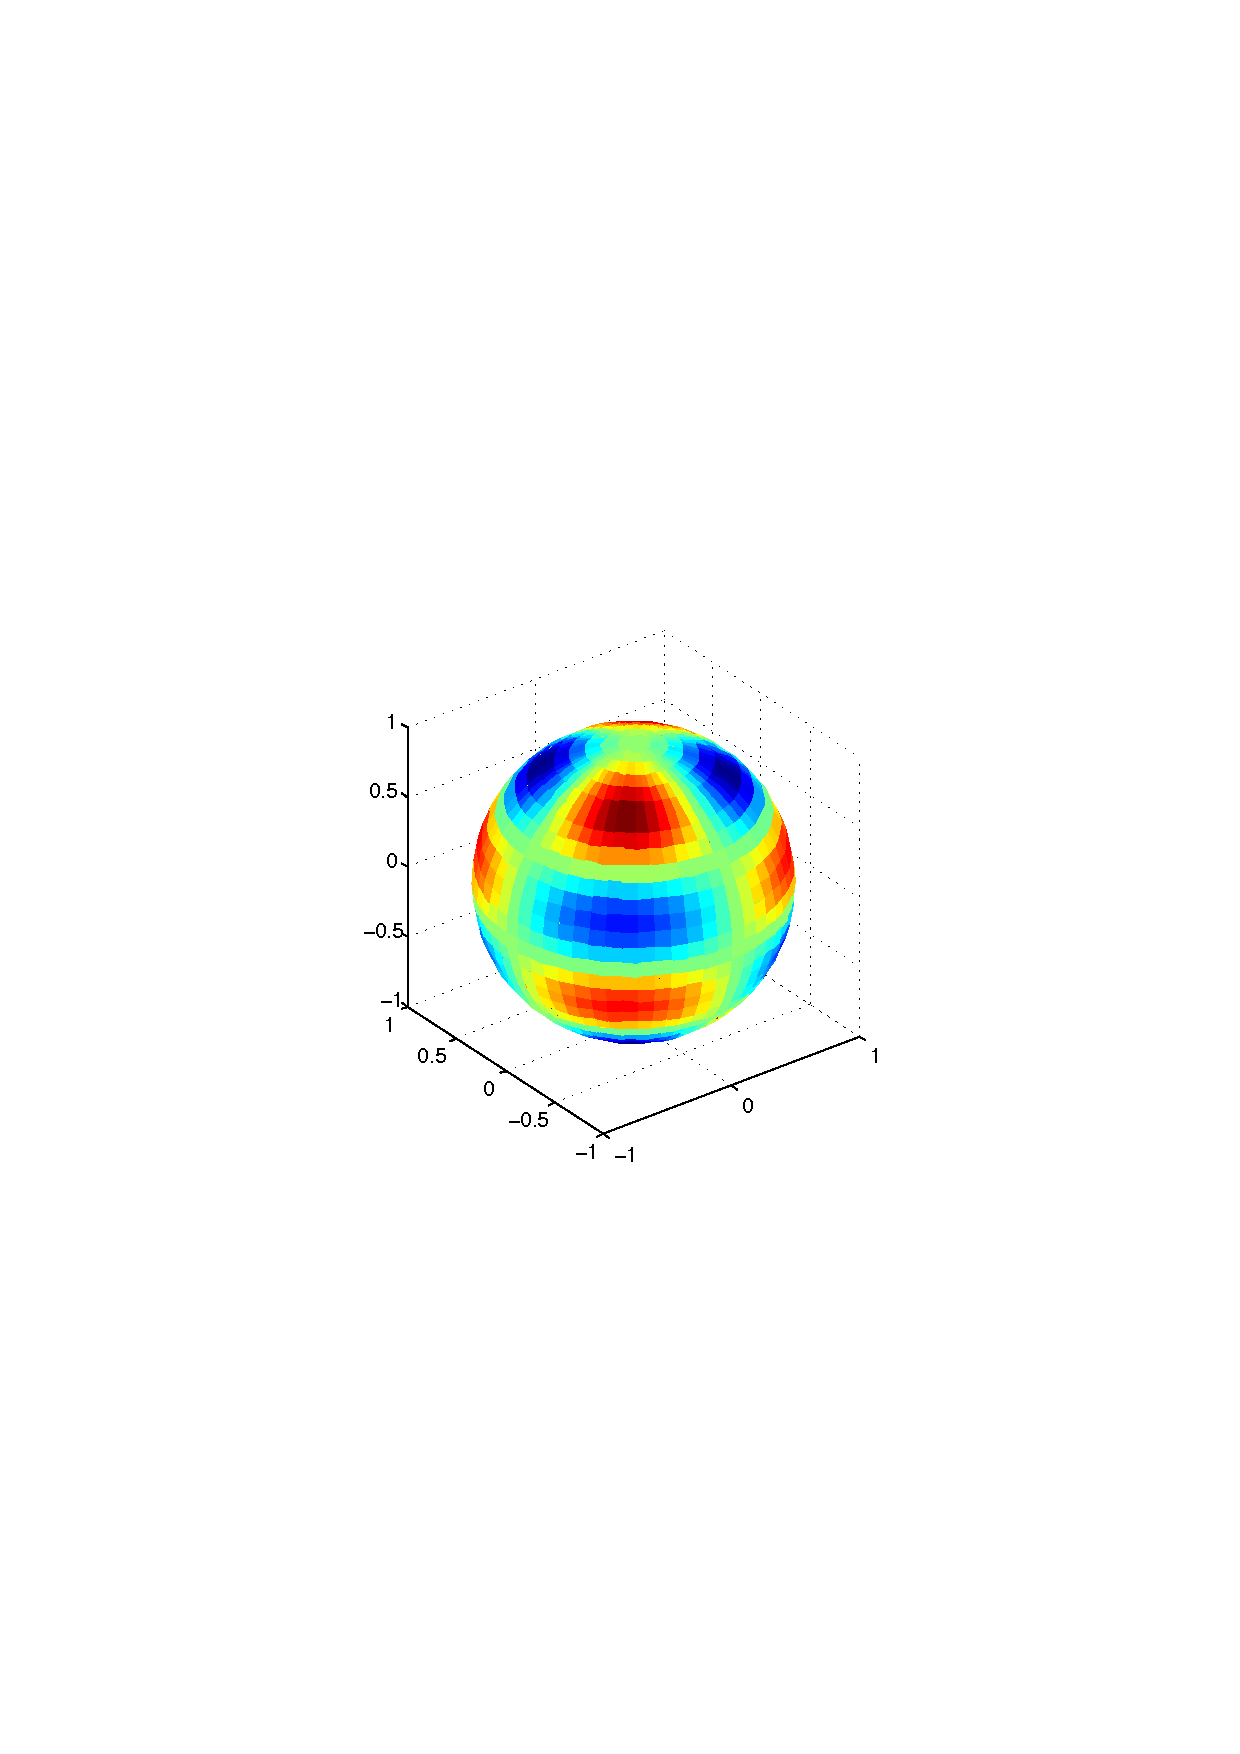
\includegraphics[width=1\textwidth]{kugel/ylm/b_5_2.pdf}
\caption{$Z_{lm}$ mit $l=5$, $m=2$}
\label{skript:zlm l=5 m=2}
\end{minipage}
\end{figure}

\begin{figure}
\begin{minipage}[hbt]{0.4\textwidth}
\centering
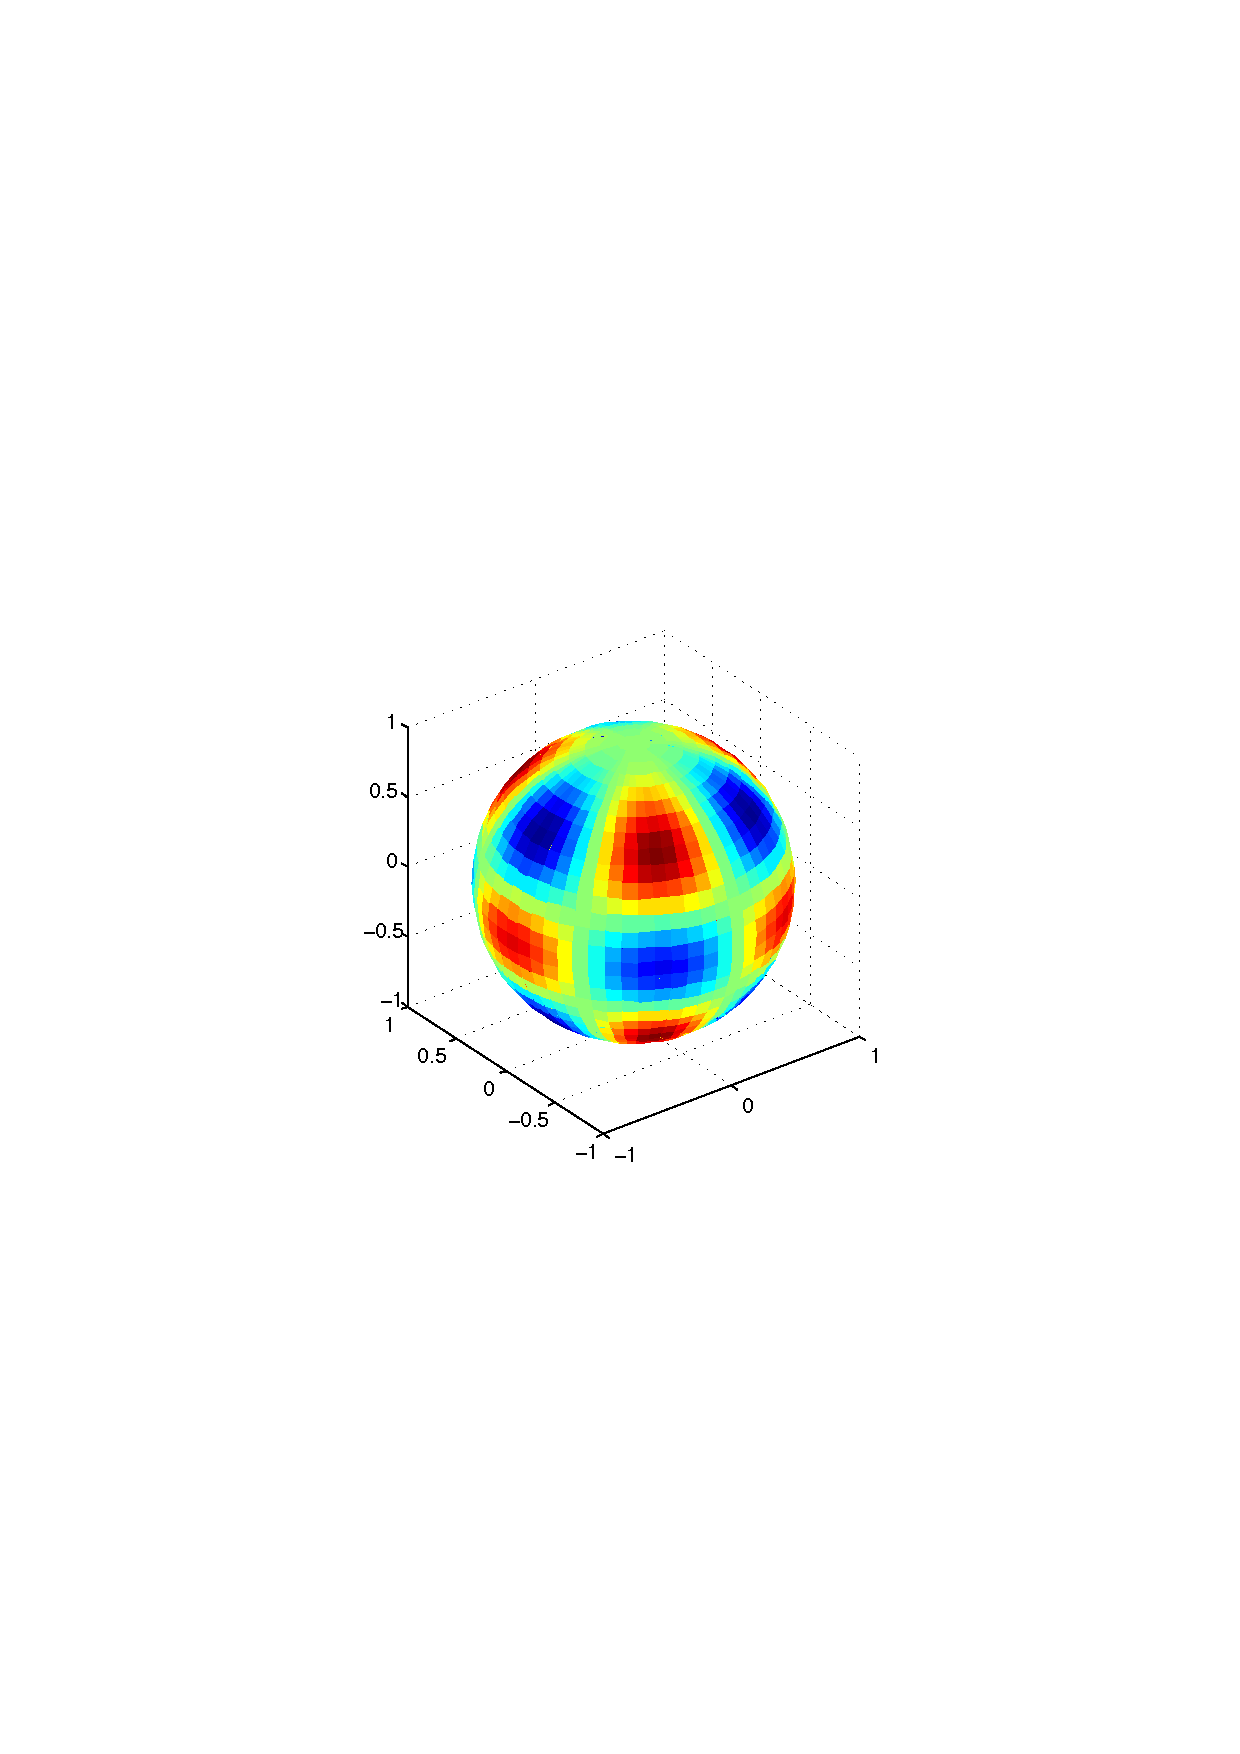
\includegraphics[width=1\textwidth]{kugel/ylm/a_5_3.pdf}
\caption{$Y_{lm}$ mit $l=5$, $m=3$}
\label{skript:ylm l=5 m=3}
\end{minipage}
\hfill
\begin{minipage}[hbt]{0.4\textwidth}
\centering
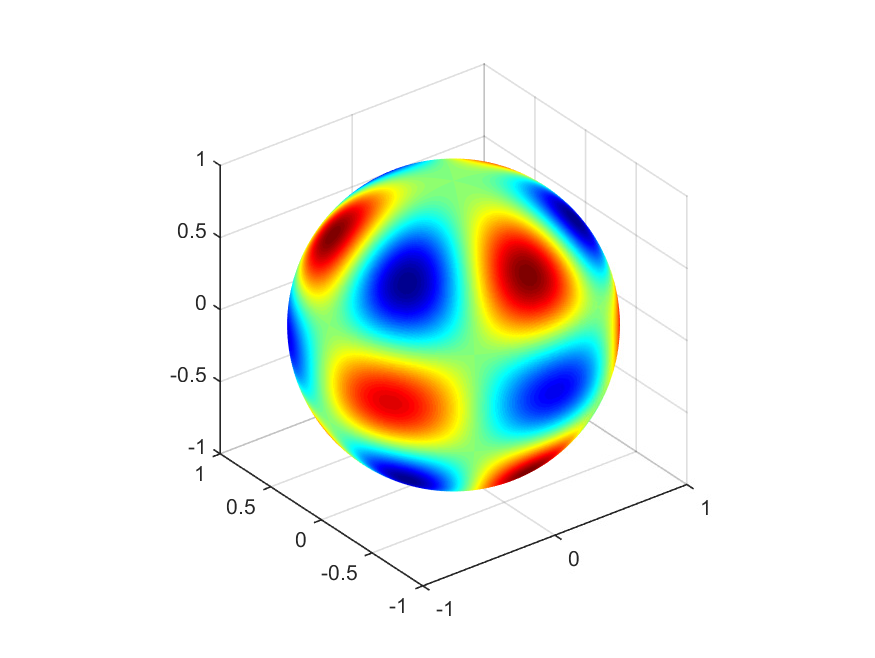
\includegraphics[width=1\textwidth]{kugel/ylm/b_5_3.pdf}
\caption{$Z_{lm}$ mit $l=5$, $m=3$}
\label{skript:zlm l=5 m=3}
\end{minipage}
\begin{minipage}[hbt]{0.4\textwidth}
\centering
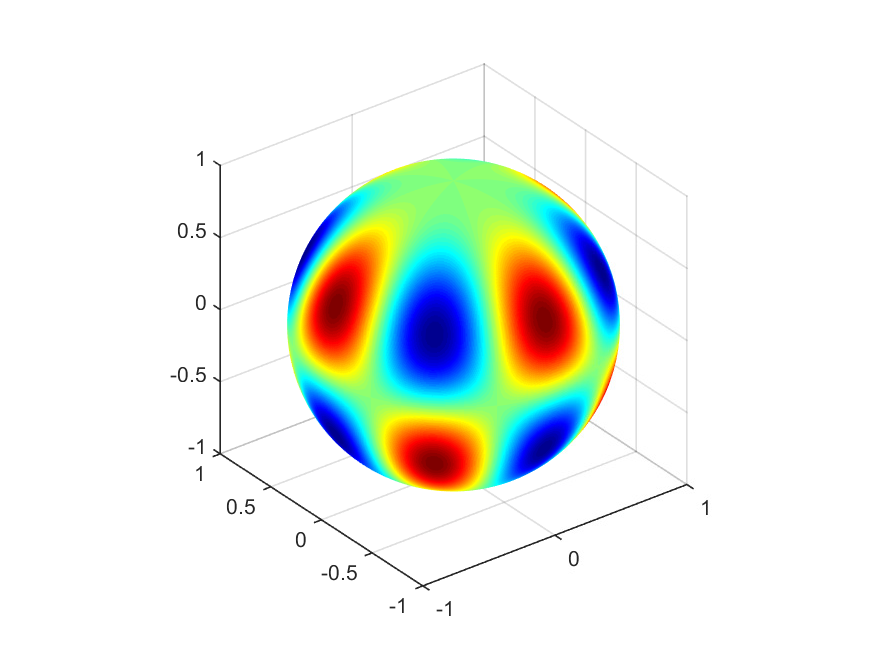
\includegraphics[width=1\textwidth]{kugel/ylm/a_5_4.pdf}
\caption{$Y_{lm}$ mit $l=5$, $m=4$}
\label{skript:ylm l=5 m=4}
\end{minipage}
\hfill
\begin{minipage}[hbt]{0.4\textwidth}
\centering
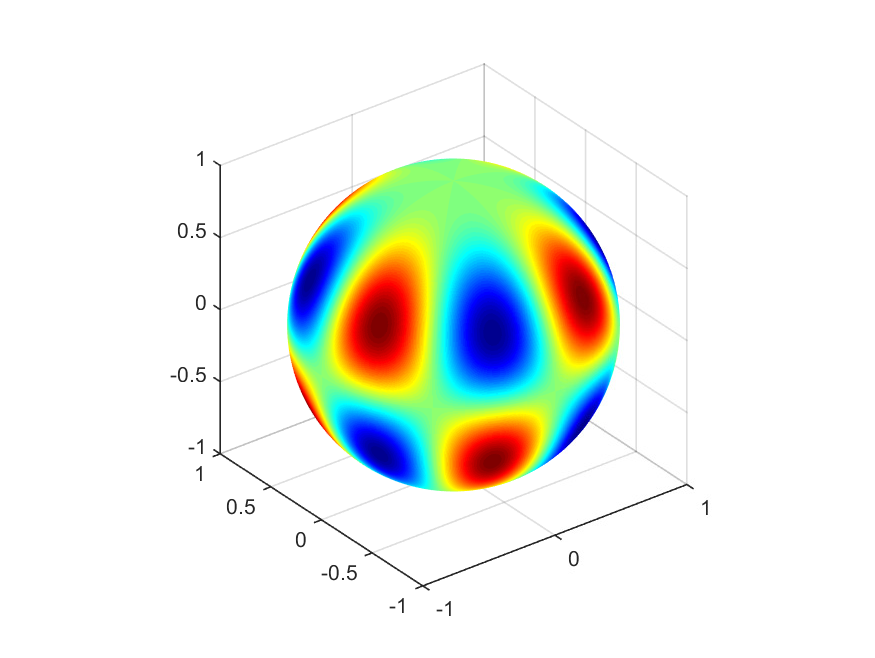
\includegraphics[width=1\textwidth]{kugel/ylm/b_5_4.pdf}
\caption{$Z_{lm}$ mit $l=5$, $m=4$}
\label{skript:zlm l=5 m=4}
\end{minipage}
\begin{minipage}[hbt]{0.4\textwidth}
\centering
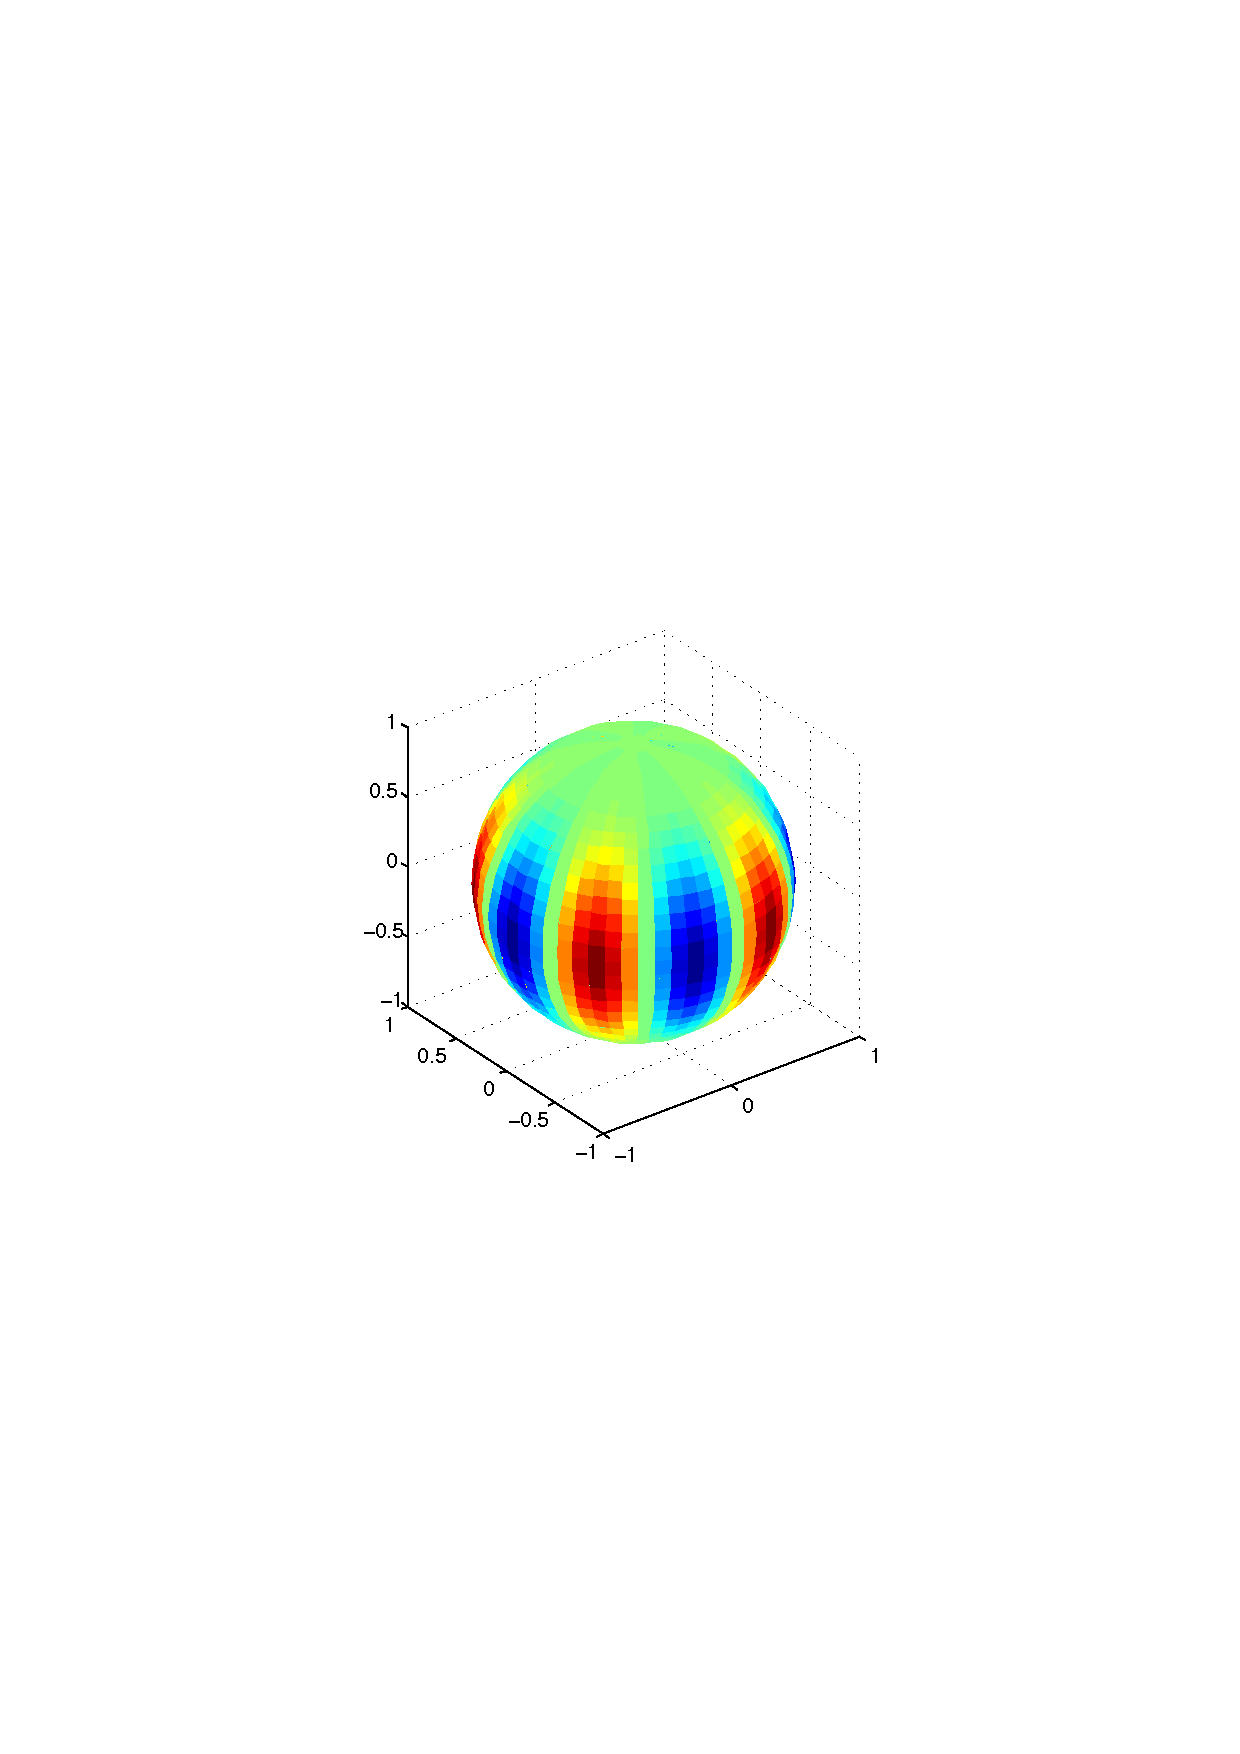
\includegraphics[width=1\textwidth]{kugel/ylm/a_5_5.pdf}
\caption{$Y_{lm}$ mit $l=5$, $m=5$}
\label{skript:ylm l=5 m=5}
\end{minipage}
\hfill
\begin{minipage}[hbt]{0.4\textwidth}
\centering
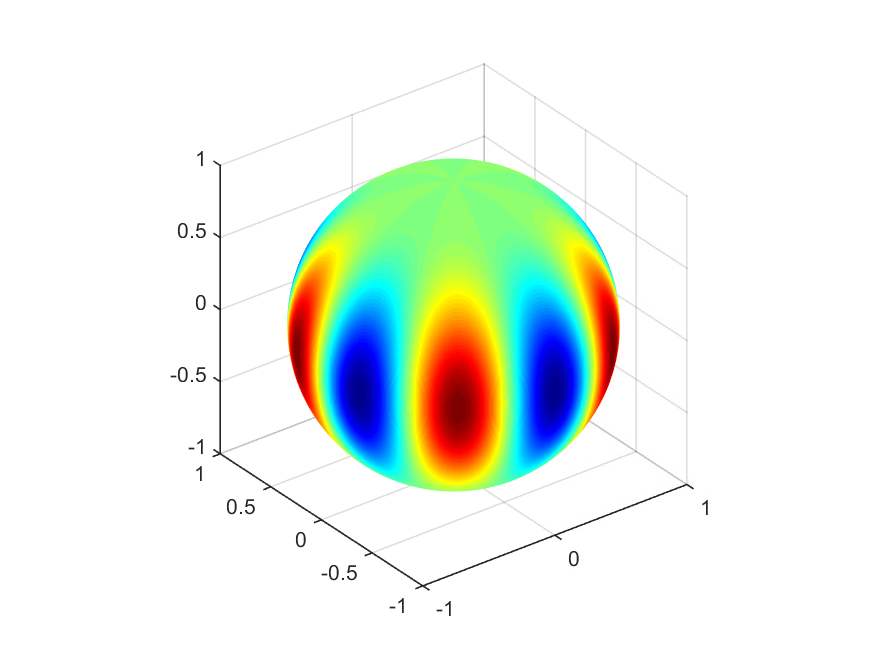
\includegraphics[width=1\textwidth]{kugel/ylm/b_5_5.pdf}
\caption{$Z_{lm}$ mit $l=5$, $m=5$}
\label{skript:zlm l=5 m=5}
\end{minipage}
\end{figure}

\subsection{Fourier-Koeffizienten}
In der klassischen Fourier-Theorie erfolgt die Berechnung der 
Fourier-Koeffizienten folgendermassen:
\begin{align*}
k&= 0: & a_{0} &= \frac{1}{2\pi} \int_{-\pi}^\pi f(x) \cdot dx
\\
&  & b_{0} &= 0
\\
k& > 0: & a_{k} &= \frac{1}{\pi} \int_{-\pi}^\pi f(x) \cdot \cos kx \cdot dx
\\
& & b_{k} &= \frac{1}{\pi} \int_{-\pi}^\pi f(x) \cdot \sin kx \cdot dx
\end{align*}
F"ur die Berechnung der Fourier-Koeffizienten auf der Kugeloberfl"ache 
verwendet man folgende Formeln:
\begin{align*}
l&=0: & a_{00} &= \frac{1}{4\pi} \int_{-\pi}^\pi \int_{0}^\pi f(\vartheta,\varphi) \cdot \sin\vartheta \cdot d\vartheta \cdot d\varphi
\\
&  & b_{00} &= 0
\\
l&\ne 0: & a_{lm} &= \frac{1}{4\pi} \int_{-\pi}^\pi \int_{0}^\pi f(\vartheta,\varphi) \cdot Y_{lm} (\vartheta, \varphi) \cdot \sin\vartheta \cdot d\vartheta \cdot d\varphi
\\
&  & b_{lm} &= \frac{1}{4\pi} \int_{-\pi}^\pi \int_{0}^\pi f(\vartheta,\varphi) \cdot Z_{lm} (\vartheta, \varphi) \cdot \sin\vartheta \cdot d\vartheta \cdot d\varphi
\end{align*}

\subsection{Berechnung der Funktion aus den Fourier-Koeffizienten}
Um eine Funktion wieder zu rekonstruieren muss man die einzelnen 
Wellenfunktionen gewichtet mit den entsprechenden Fourier-Koeffizienten 
wieder aufsummieren.

In der klassischen Fourier-Theorie wird folgendermassen vorgegangen:
\begin{equation}
\begin{aligned}
f(x)&=a_0 + \sum_{n=0}^\infty \Big( a_k \cdot \cos kx + b_k \sin kx \Big)
\end{aligned}
\end{equation}
Will man eine Funktion auf der Kugeloberfl"ache wieder rekonstruieren 
muss man folgende Formel verwenden:
\begin{equation}
\begin{aligned}
f(\vartheta, \varphi) &= a_{00} + \sum_{l=1}^\infty \sum_{m=0}^l \Big( a_{lm} \cdot Y_{lm}(\vartheta, \varphi) + b_{lm} \cdot Z_{lm}(\vartheta, \varphi) \Big)
\end{aligned}
\end{equation}
\subsection{Kugelspektrum}
Um das komplexe Amplitudenspektrum darstellen zu k"onnen muss man die
Sinus- und Kosinus-Koeffizienten zusammenfassen.
\begin{align*}
c_k= \sqrt{a^2_{k}+b^2_{k}}
\end{align*}
Man kann ein Kugelspektrum analog zum komplexen Amplitudenspektrum 
darstellen. 
Dabei muss man die Summe der Quadrate $a$- und der $b$-Koeffizienten mit 
dem gleichen Index $l_m$ bilden. Anschliessend muss man alle 
mit dem selben Index $l$ aufsummieren und von den daraus resultierenden 
Koeffizienten die Wurzel ziehen. Man erh"alt 
\begin{align*}
c_l= \sqrt{\sum_{m=0}^l (a^2_{lm}+b^2_{lm})} .
\end{align*}
Weder das komplexe Amplitudenspektrum noch das Kugelspektrum enthalten 
Ortsinformationen. 
Dies bedeutet, dass diese Spektren unabh"angig von der
Phasenlage konstant bleiben, da Ortsinformationen im 
Phasendiagramm enthalten sind.

\subsection{Numerische Berechnung des Kugelspektrums}
Allf"allige Abweichungen in unseren Darstellungen sind auf die 
numerischen Berechnungen zur"uckzuf"uhren, da wir die Integrale  
mit einer Riemann-Summe approximiert haben.
Qualitativ sind jedoch alle Ergebnisse korrekt. 

\section{Spektrum einer Rechteckfunktion}
\rhead{Spektrum einer Rechteckfunktion}
Um aufzuzeigen, dass das komplexe Amplitudenspektrum unabh"angig von 
der Phasenlage konstant bleibt, haben wir eine wandernde 
Rechteckfunktion generiert. 
Dazu haben wir die Parameter $u$ und $v$ der Formel 
(\ref{skript:Rechteckfunktion Formel})
unter der Bedingung: $u - v$ = $\pi$ variiert.
Damit haben wir sicher gestellt, dass die Abmessungen unserer 
Rechteckfunktion konstant bleiben und sich nur die Phasenlage "andert.
In Abbildung \ref{skript:Spektrum1} sieht man eine solche 
Rechteckfunktion in vier verschiedenen Phasenlagen mit den zugeh"origen 
komplexen Amplitudenspektren. 
Es ist zu beachten, dass beim komplexen Amplitudenspektrum der 
Fourier-Koeffizient $c_0$ aus Darstellungsgr"unden abgeschnitten wurde.

Um die Analogie f"ur eine Funktion auf der Kugeloberfl"ache aufzuzeigen, 
haben wir den Vektor $\vec{c}$ variiert indem wir die Winkel $\vartheta_c$
und $\varphi_c$ aus der Formel (\ref{skript:Vektor c Formel}) 
kontinuierlich ver"andert haben. 
Mittels dieser "Anderung haben wir die Phasenlage variiert.
 
Um zu garantieren, dass die Abmessung unserer Funktion auf der 
Kugeloberl"ache konstant bleibt, haben wir die Bedingung gestellt,
dass der Parameter $w$ der Formel (\ref{skript:Kugelfunktion Formel}) 
konstant auf 0 gesetzt ist. 
Dadurch haben wir eine Funktion erhalten, welche auf der einen 
H"alfte der Kugeloberfl"ache den Funktionswert 1 und auf der 
anderen H"alfte den Funktionswert 0 besitzt. 
Wie schon bei der Rechteckfunktion sieht man, in Abbildung 
\ref{skript:Spektrum2}  
unsere Kugelfunktion in vier verschiedenen Phasenlagen mit den 
zugeh"origen Kugelspektren.
Die Kugelspektren sind auch hier praktisch identisch. 

Zu der besseren Veranschaulichung, ist dem Buch eine CD 
beigelegt.
Diese CD enth"alt je ein Video, dass eine wandernde 
Rechteckfunktion mit dem komplexen Amplitudenspektrum zeigt und
ausserdem eine rotierende Funktion auf der Kugeloberfl"ache mit 
dem  dazugeh"origen Kugelspektrum. 
Zus"atzlich sieht man in den Videos auch
die sich st"andig "andernden $a$- und $b$-Koeffizienten. Bei der 
Rechteckfunktion ist auch noch das Phasendiagramm dargestellt.

\begin{figure}
\centering
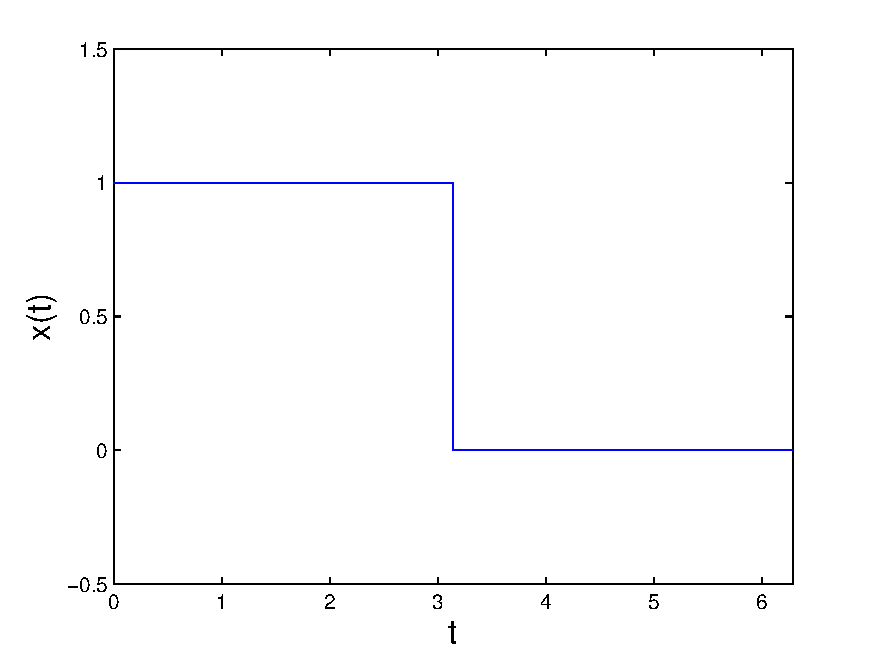
\includegraphics[width=0.45\textwidth]{kugel/kSpektrum/Rechteck1_1.pdf}
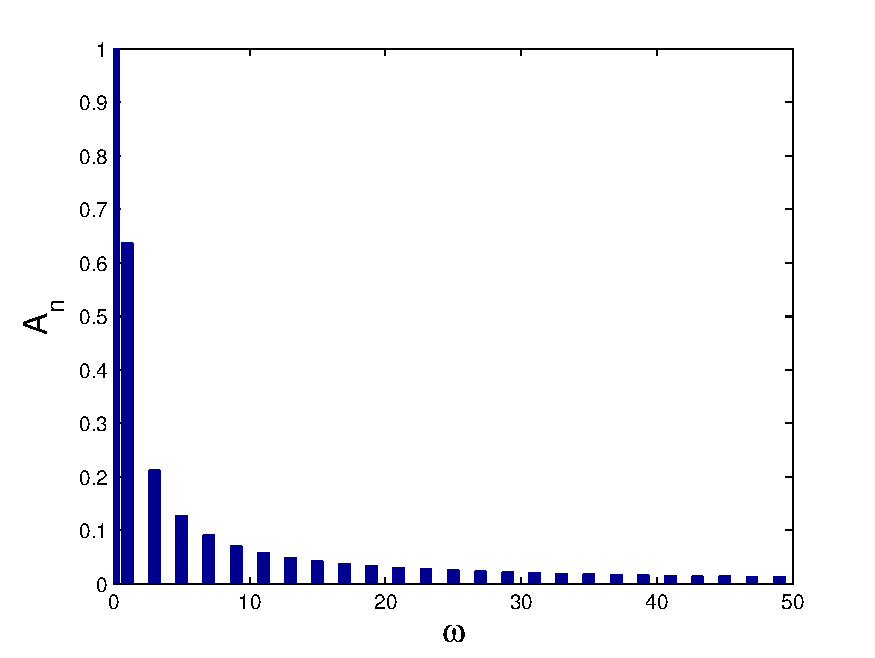
\includegraphics[width=0.45\textwidth]{kugel/kSpektrum/Rechteck1_2.pdf}
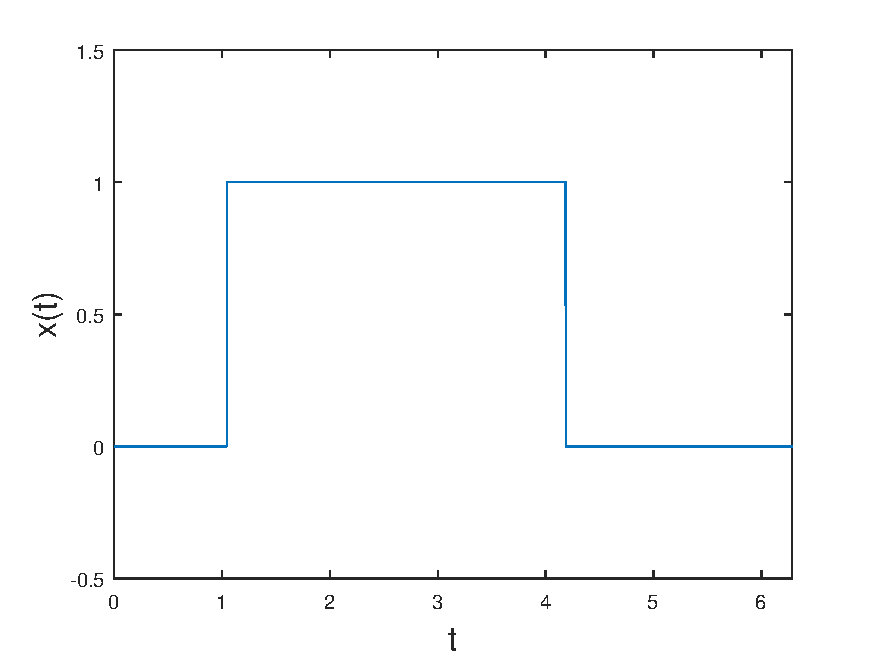
\includegraphics[width=0.45\textwidth]{kugel/kSpektrum/Rechteck2_1.pdf}
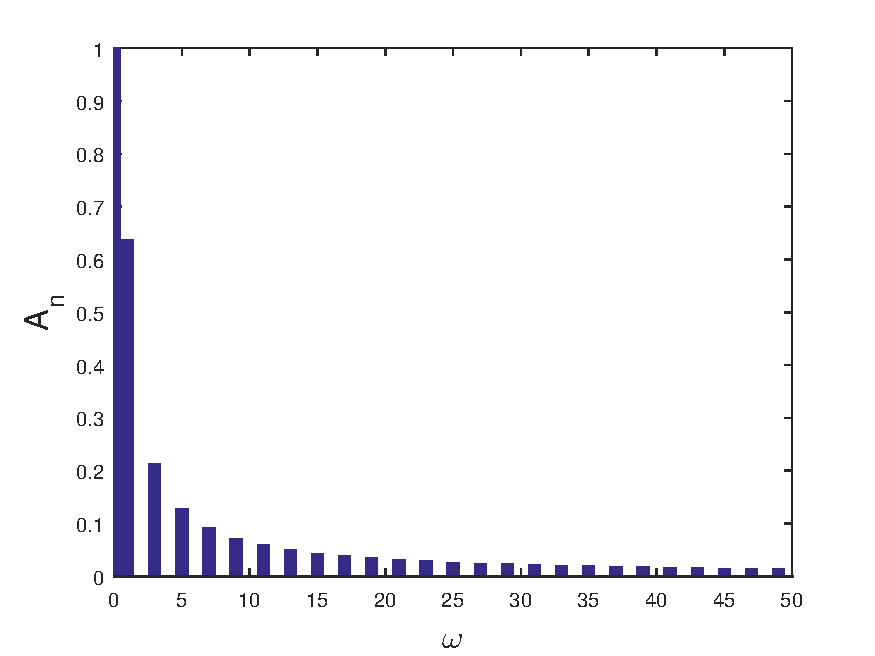
\includegraphics[width=0.45\textwidth]{kugel/kSpektrum/Rechteck2_2.pdf}
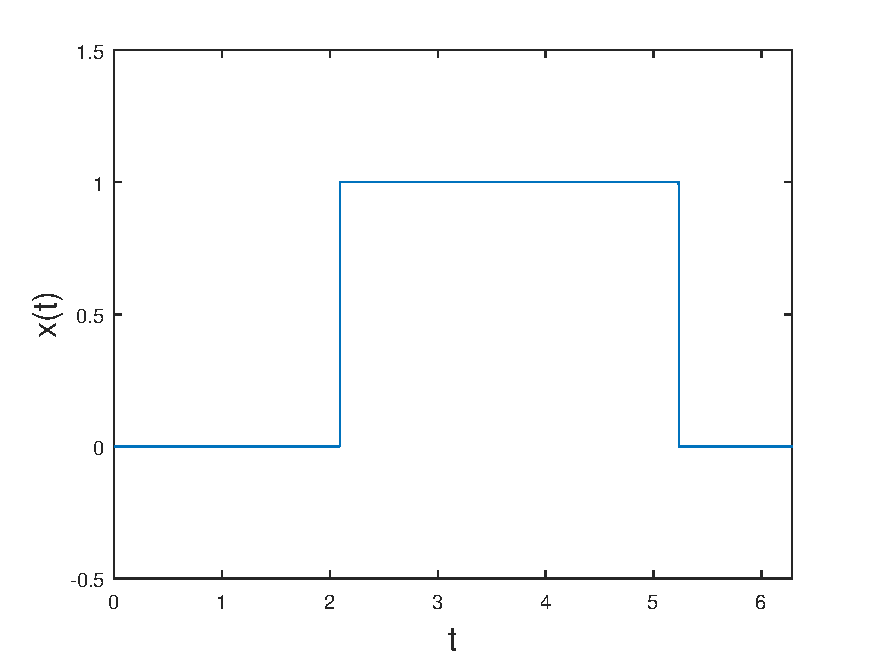
\includegraphics[width=0.45\textwidth]{kugel/kSpektrum/Rechteck3_1.pdf}
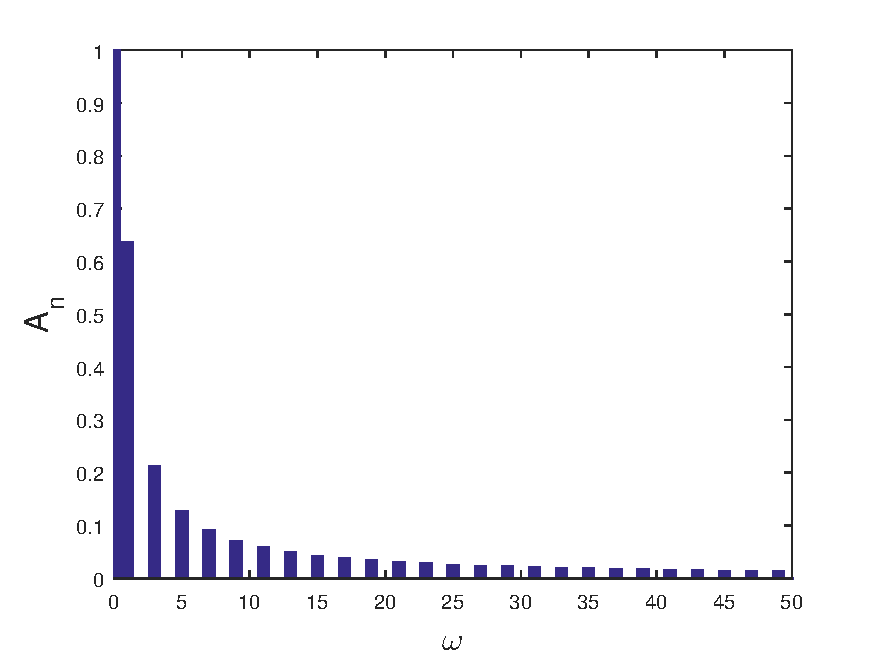
\includegraphics[width=0.45\textwidth]{kugel/kSpektrum/Rechteck3_2.pdf}
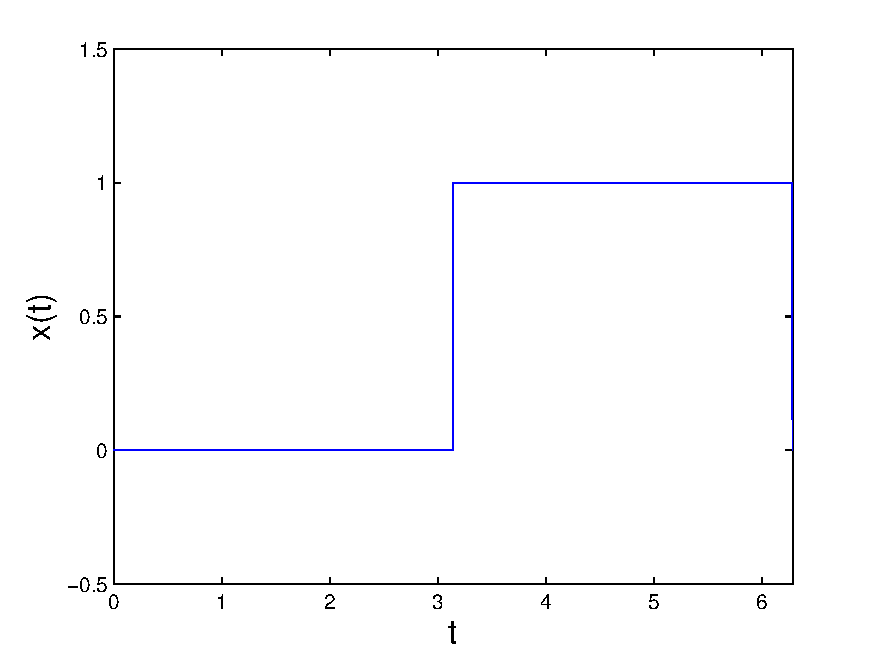
\includegraphics[width=0.45\textwidth]{kugel/kSpektrum/Rechteck4_1.pdf}
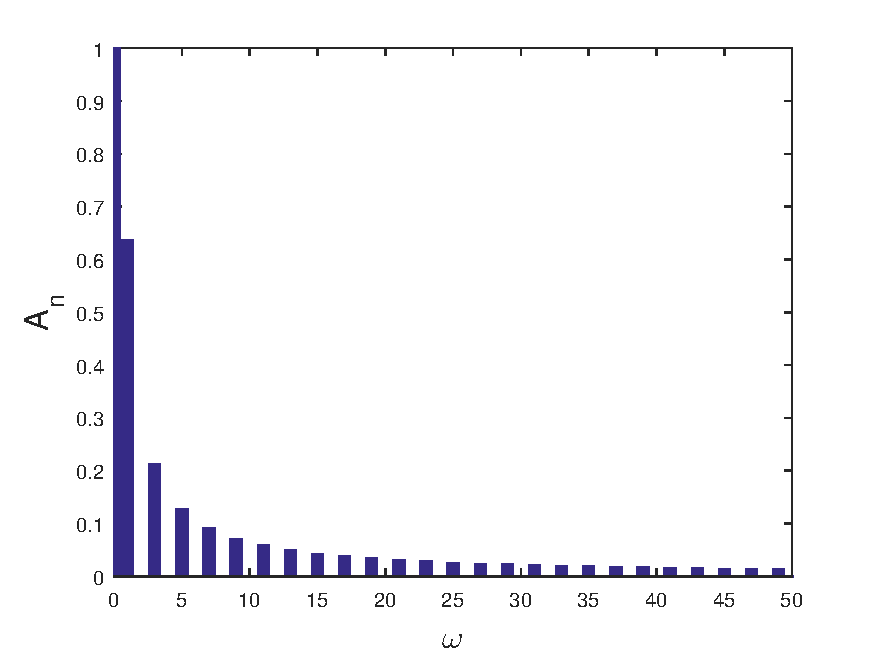
\includegraphics[width=0.45\textwidth]{kugel/kSpektrum/Rechteck4_2.pdf}
\caption{Wandernde Rechteckfunktion
\label{skript:Spektrum1}}
\end{figure}

\begin{figure}
\centering
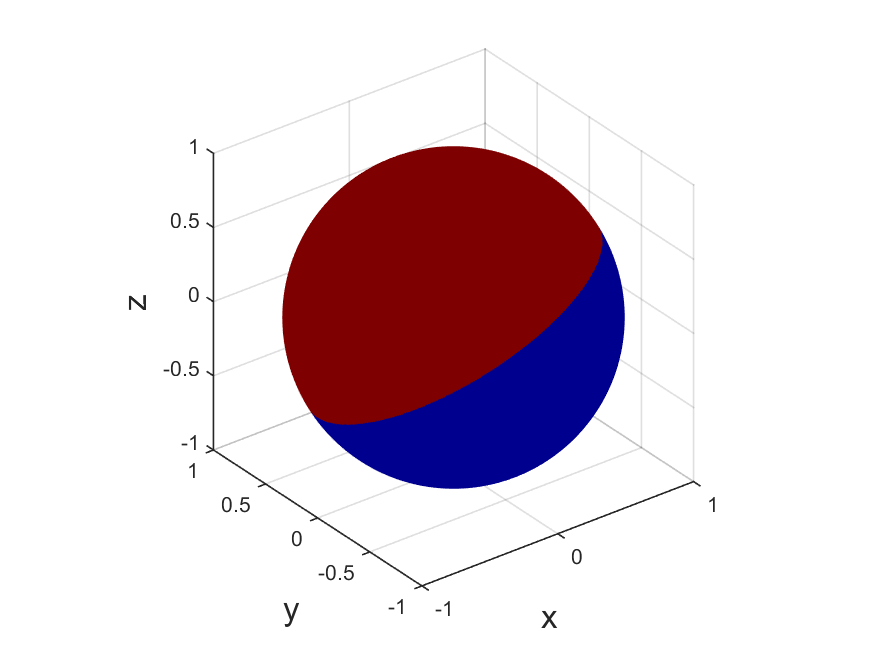
\includegraphics[width=0.45\textwidth]{kugel/kSpektrum/Kugel_1_1.pdf}
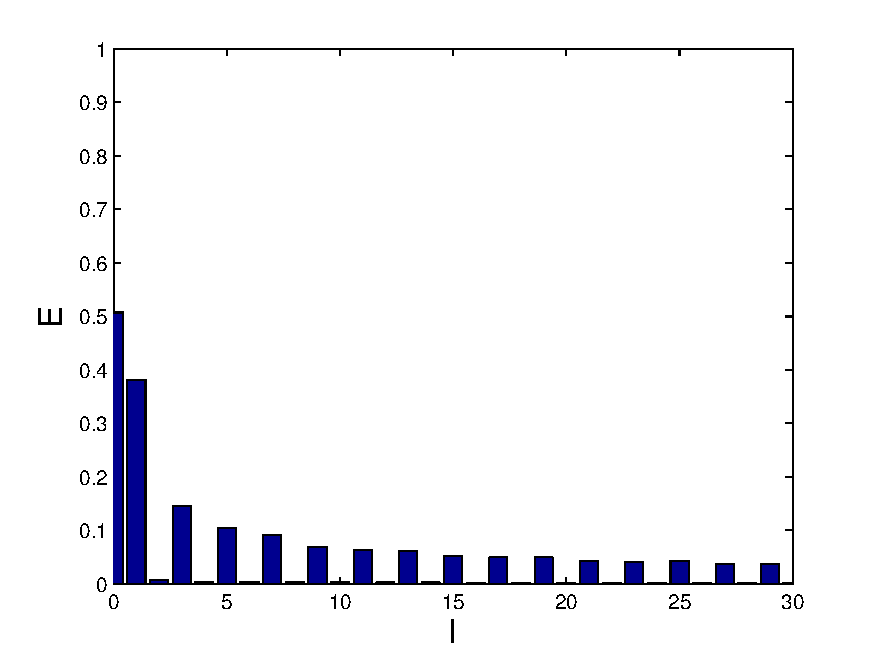
\includegraphics[width=0.45\textwidth]{kugel/kSpektrum/Kugel_1_2.pdf}
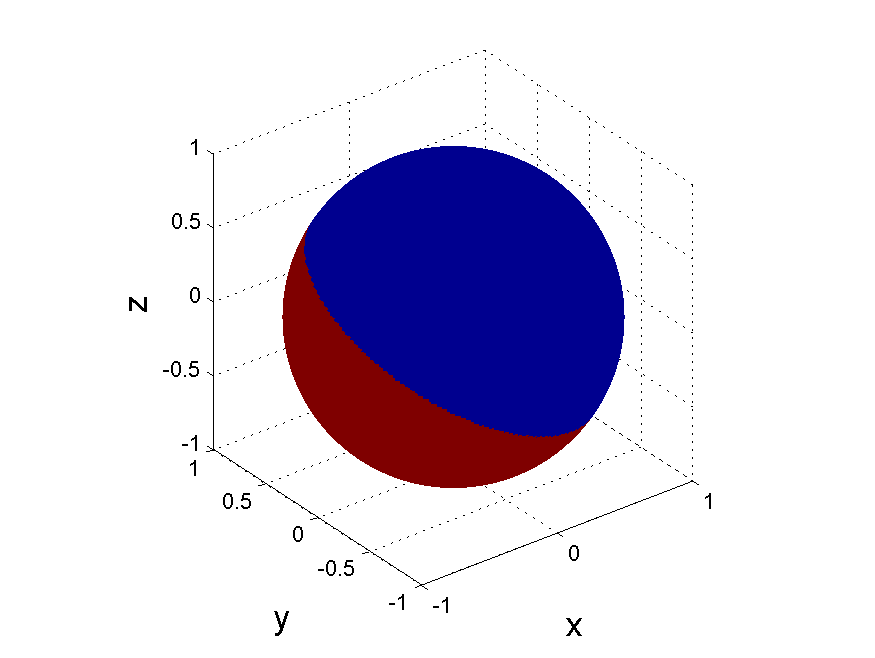
\includegraphics[width=0.45\textwidth]{kugel/kSpektrum/Kugel_2_1.pdf}
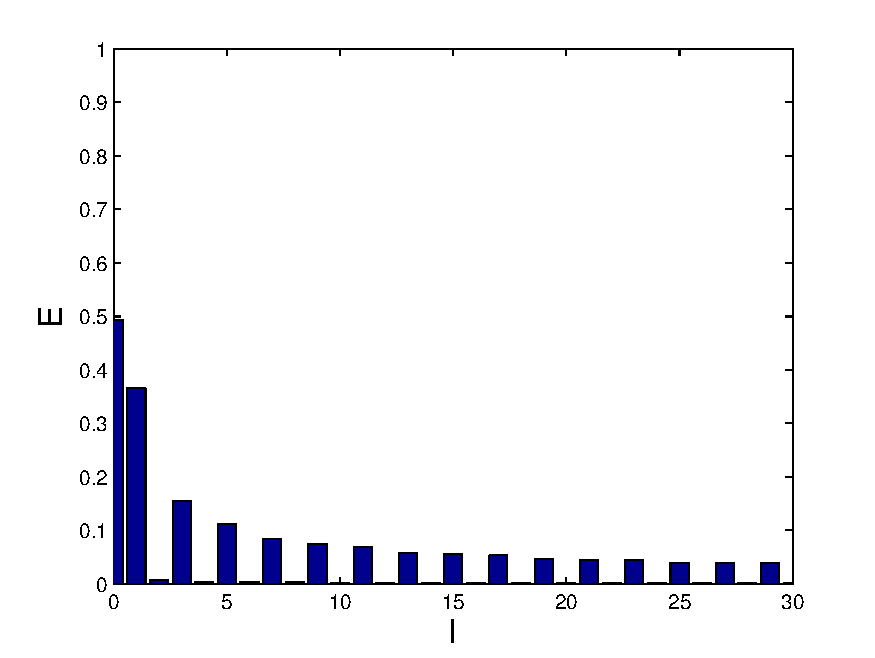
\includegraphics[width=0.45\textwidth]{kugel/kSpektrum/Kugel_2_2.pdf}
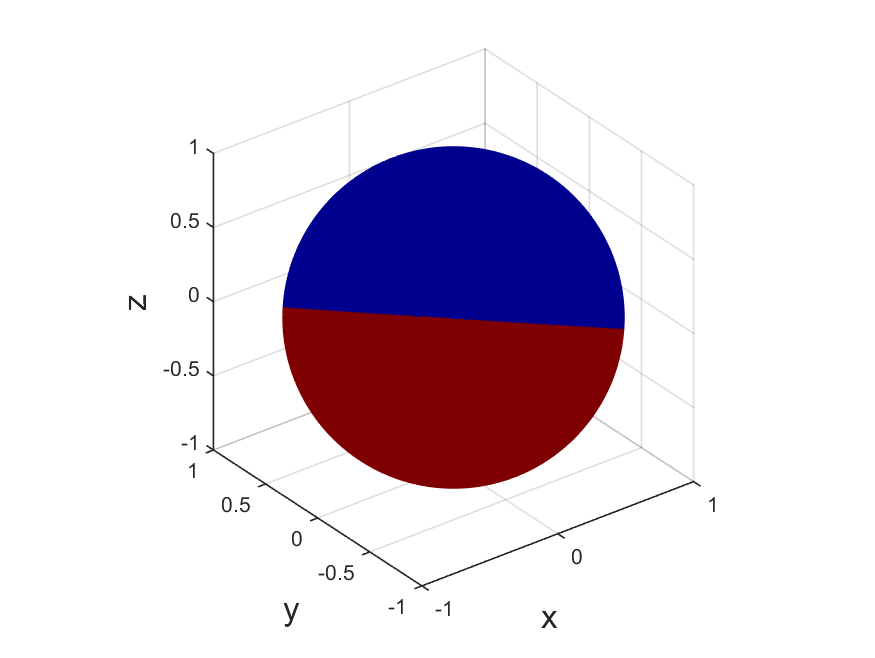
\includegraphics[width=0.45\textwidth]{kugel/kSpektrum/Kugel_3_1.pdf}
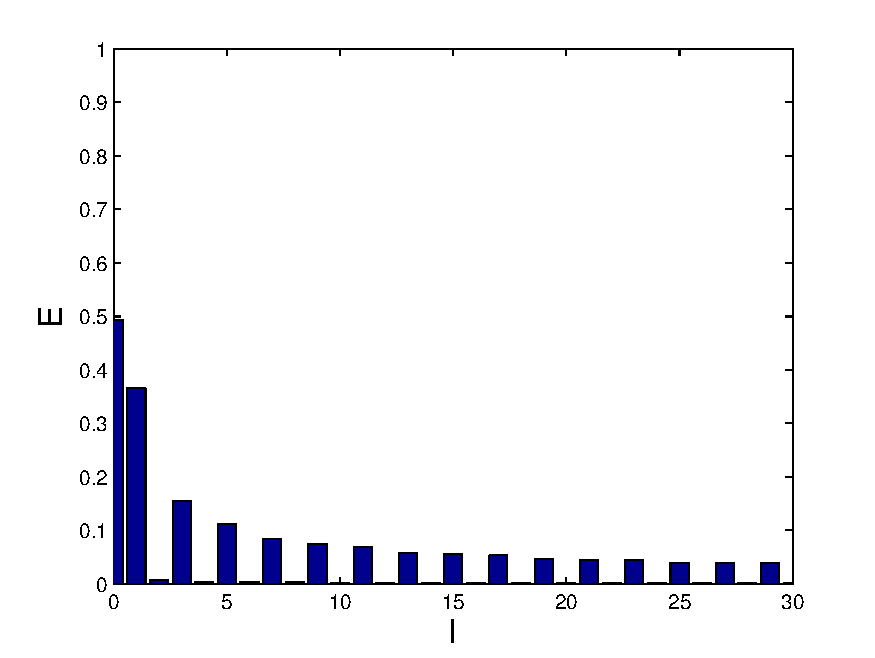
\includegraphics[width=0.45\textwidth]{kugel/kSpektrum/Kugel_3_2.pdf}
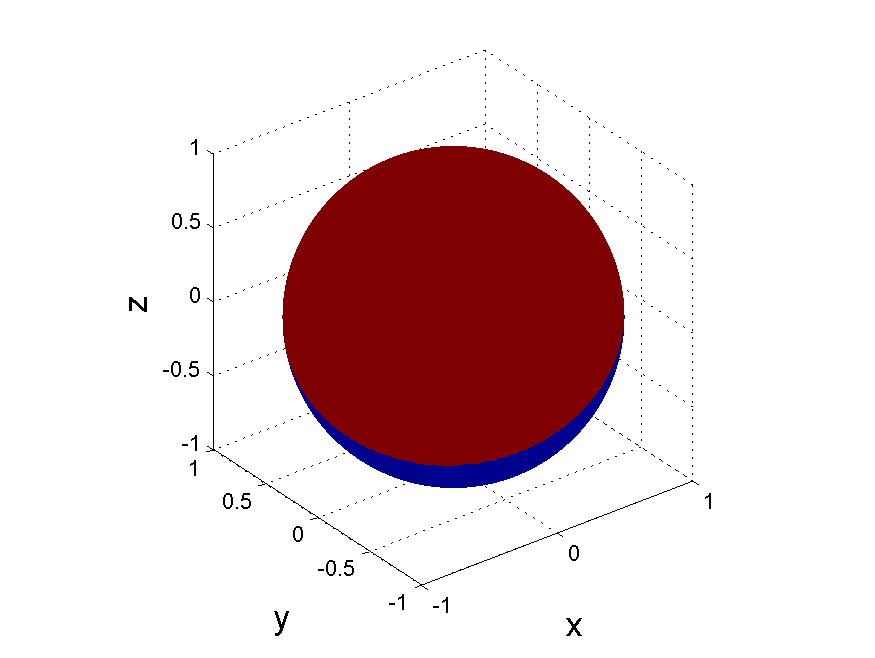
\includegraphics[width=0.45\textwidth]{kugel/kSpektrum/Kugel_4_1.pdf}
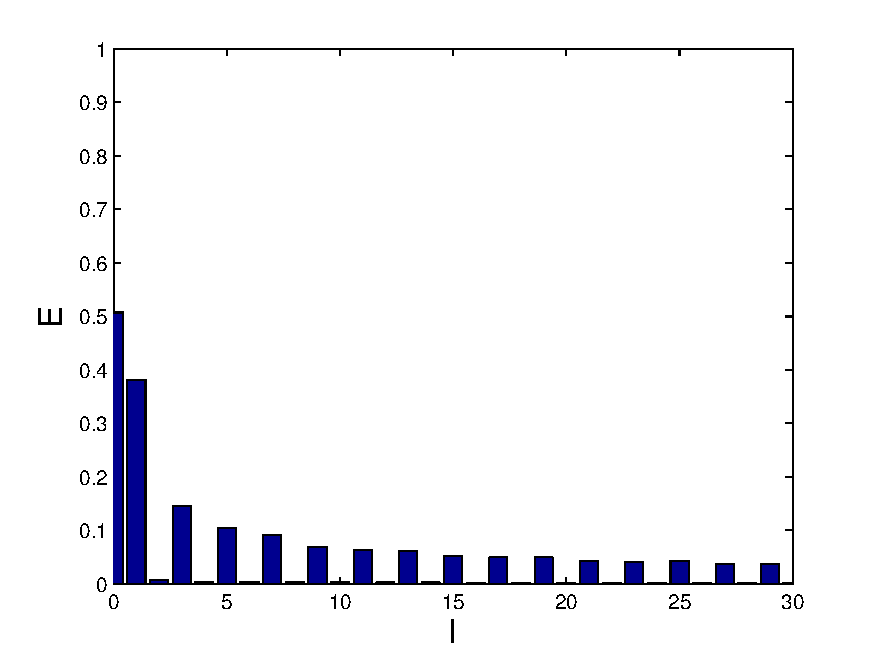
\includegraphics[width=0.45\textwidth]{kugel/kSpektrum/Kugel_4_2.pdf}
\caption{Rotierende Funktion auf der Kugeloberfl"ache
\label{skript:Spektrum2}}
\end{figure}

\section{Dirac Stoss und konstante Funktion}
\rhead{Dirac Stoss und konstante Funktion}

In diesem Abschnitt m"ochten wir aufzeigen, dass im Falle eines 
unendlich schmalen Rechtecksignals, wie auch einem unendlich kleinen 
Kreisabschnitt auf der Kugeloberfl"ache mit dem Funktionswert 1 beim 
komplexen Amplitudenspektrum und dem Kugelspektrum alle 
Fourier-Koeffizienten gleich stark gewichtet sind. 
Analysiert man hingegen ein Rechtecksignal oder eine Funktion auf der 
Kugeloberfl"ache, dass "uberall den Funktionswert 1 besitzt, ist nur 
noch der Fourier-Koeffizient $c_0$ $\neq$ 0.

Um dies f"ur das Rechtecksignal darzustellen, hielten wir den Parameter
$u$ aus der Formel (\ref{skript:Rechteckfunktion Formel}) konstant auf 0 
und variierten den Parameter $v$ derselben Formel von 0 bis 2$\pi$. 
Dadurch erhielten wir eine immer breiter werdende Rechteckfunktion. 
In Abbildung \ref{skript:Dirac1} sieht man die Rechteckfunktion in 
vier verschiedene Breiten, sowie die zugeh"origen komplexen 
Amplitudenspektren. 
Wie auch schon bei den komplexen Amplitudenspektren in Abbildung
\ref{skript:Spektrum1} wurde der Fourier-Koeffizient $c_0$ aus 
Darstellungsgr"unden abgeschnitten.

Um dies analog auf der Kugeloberfl"ache zu illustrieren, haben 
wir die Winkel $\vartheta_c$ und $\varphi_c$ aus der Formel 
(\ref{skript:Vektor c Formel}) konstant  gehalten und haben lediglich 
den Parameter $w$ aus der Formel (\ref{skript:Kugelfunktion Formel}) 
zwischen von 1 bis $-1$ variiert. 
Dadurch wurde der Kreisabschnitt, der den Funktionswert 1 hat, immer 
gr"oösser. 
In Abbildung \ref{skript:Dirac2} sieht man die Funktion auf der 
Kugeloberfl"ache mit vier verschieden grossen Kreisabschnitten, welche 
den Funktionswert 1 haben mit den zugeh"origen Kugelspektren. Auch
hier sieht man den "Ubergang von einem Dirac zu einem wesentlichen 
konstanten Spektrum.

Um auch dies noch besser zu veranschaulichen, sind auf der CD zum Buch 
je ein Video mit einer immer breiter werdenden Rechteckfunktion mit dem 
komplexen Amplitudenspektrum, sowie eine Funktion auf der 
Kugeloberfl"ache mit immer gr"osser werdendem Kreisabschnitt mit 
Funktionswert 1 mit dem zugeh"origen Kugelspektrum zu sehen. 
Wie bei den Videos, die bereits im letzten Abschnitt erw"ahnt wurden, 
sind ebenfalls die $a$- und $b$-Koeffizienten sowie bei der 
Rechteckfunktion das Phasendiagramm zu sehen.
\begin{figure}
\centering
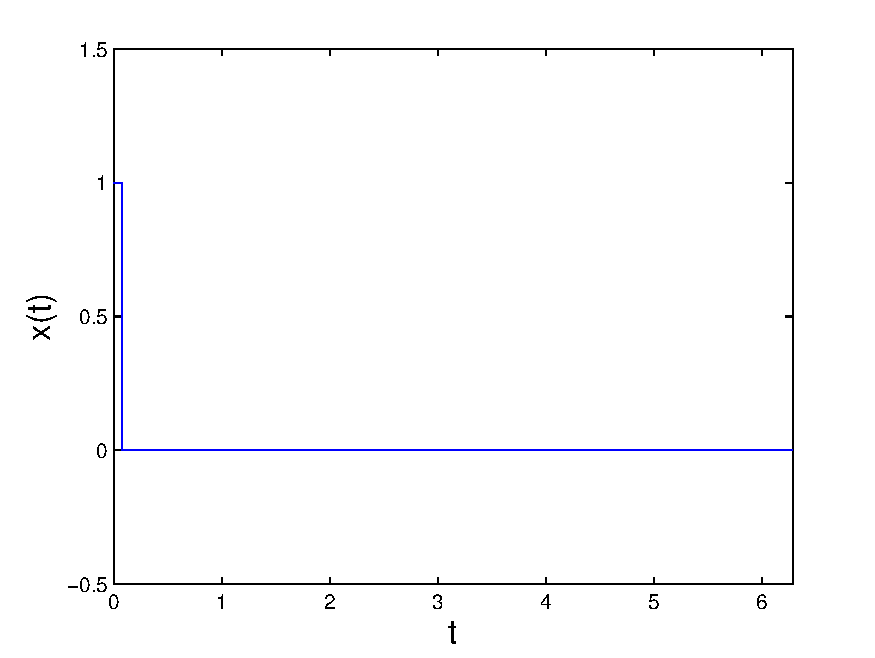
\includegraphics[width=0.45\textwidth]{kugel/Dkonstant/Rechteck1_1.pdf}
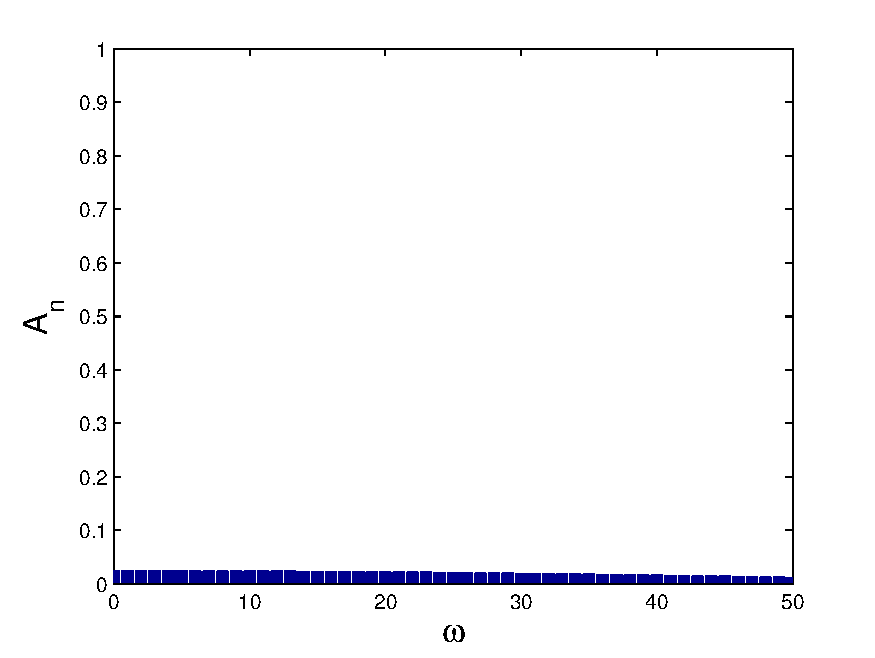
\includegraphics[width=0.45\textwidth]{kugel/Dkonstant/Rechteck1_2.pdf}
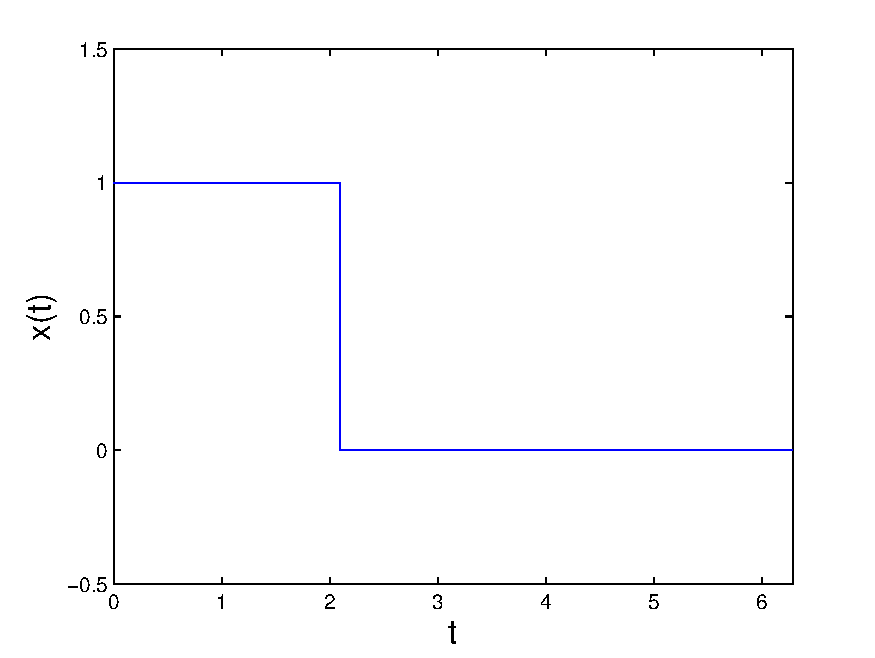
\includegraphics[width=0.45\textwidth]{kugel/Dkonstant/Rechteck2_1.pdf}
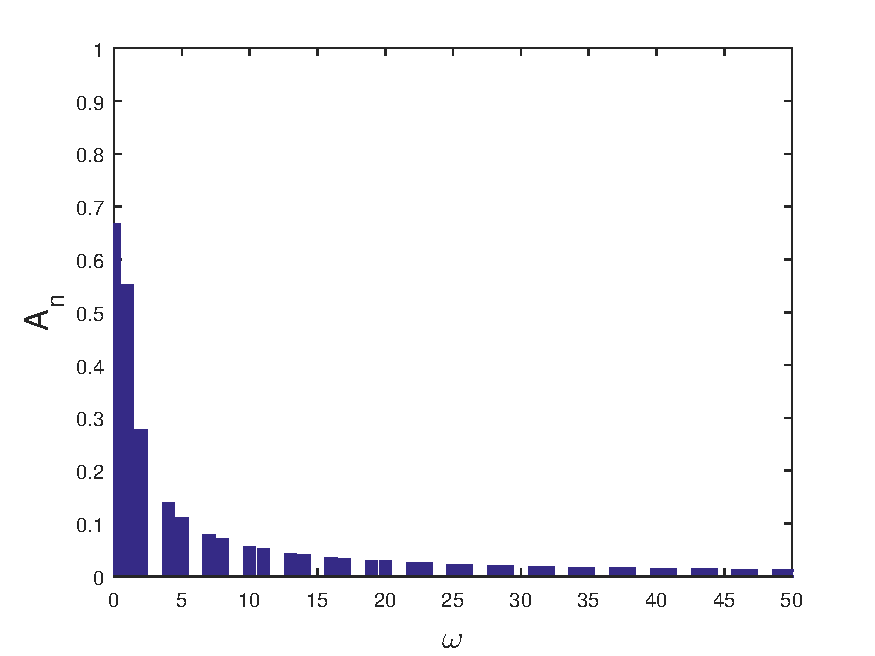
\includegraphics[width=0.45\textwidth]{kugel/Dkonstant/Rechteck2_2.pdf}
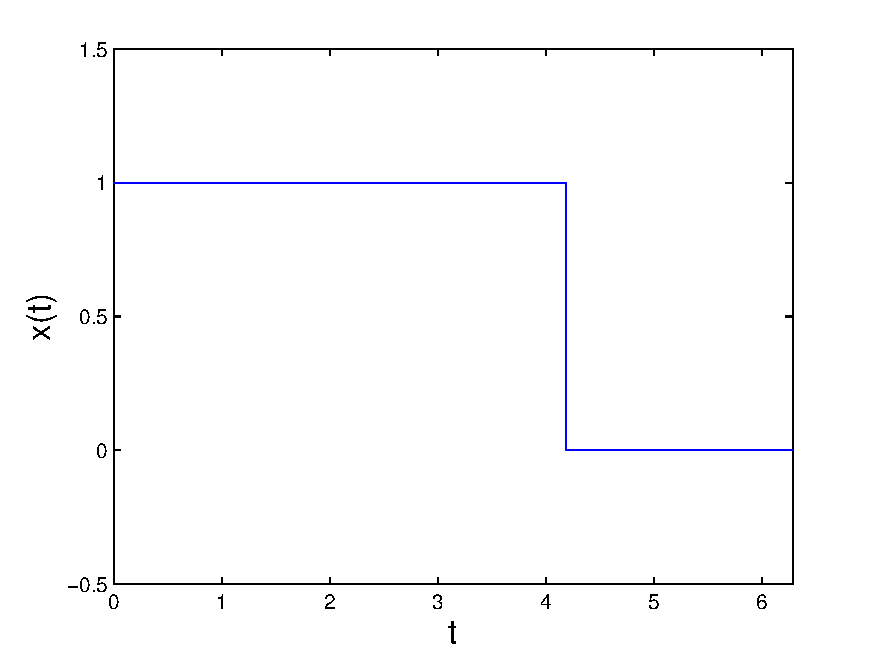
\includegraphics[width=0.45\textwidth]{kugel/Dkonstant/Rechteck3_1.pdf}
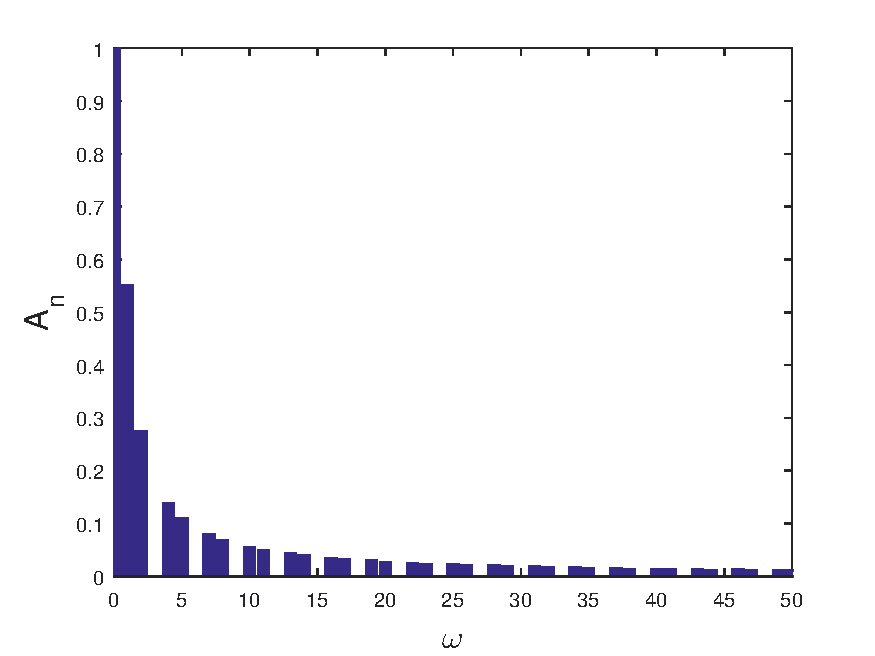
\includegraphics[width=0.45\textwidth]{kugel/Dkonstant/Rechteck3_2.pdf}
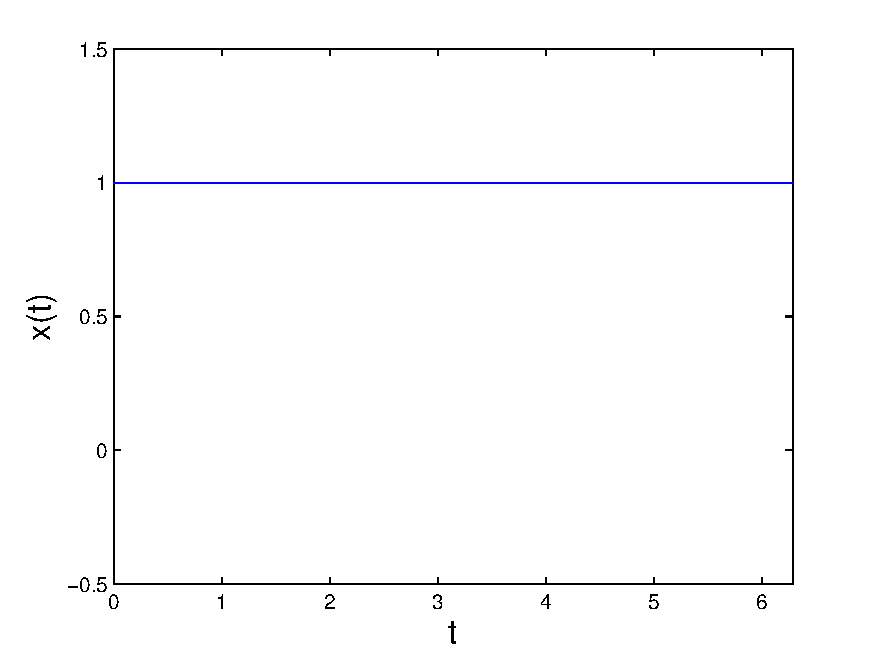
\includegraphics[width=0.45\textwidth]{kugel/Dkonstant/Rechteck4_1.pdf}
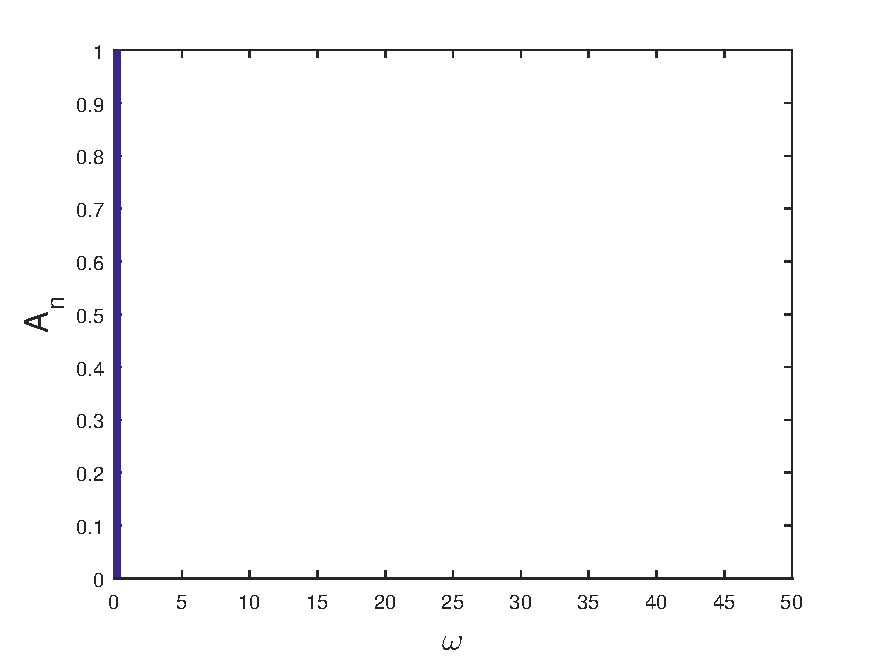
\includegraphics[width=0.45\textwidth]{kugel/Dkonstant/Rechteck4_2.pdf}
\caption{Breiter werdende Rechteckfunktion
\label{skript:Dirac1}}
\end{figure}

\begin{figure}
\centering
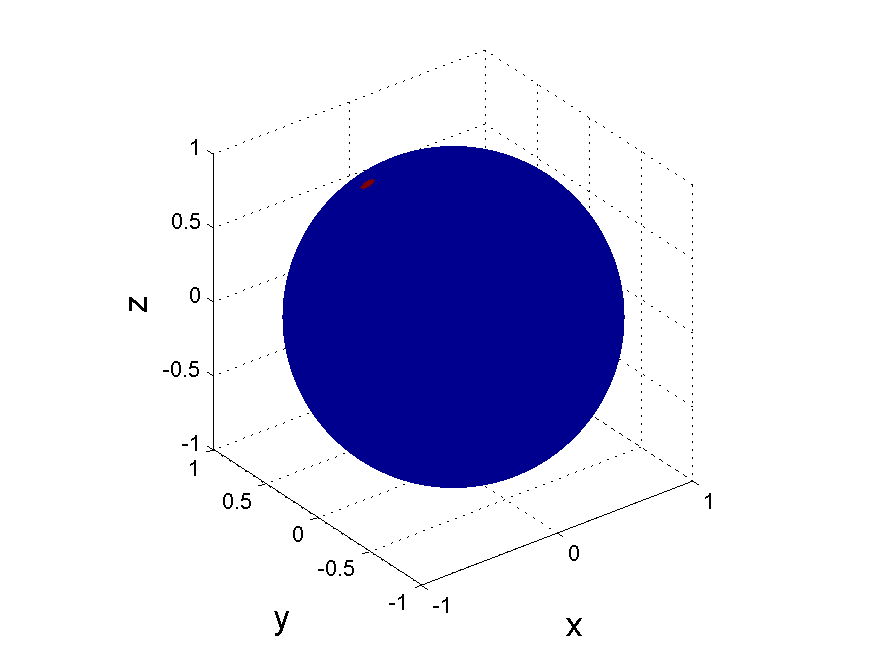
\includegraphics[width=0.45\textwidth]{kugel/Dkonstant/Kugel1_1.pdf}
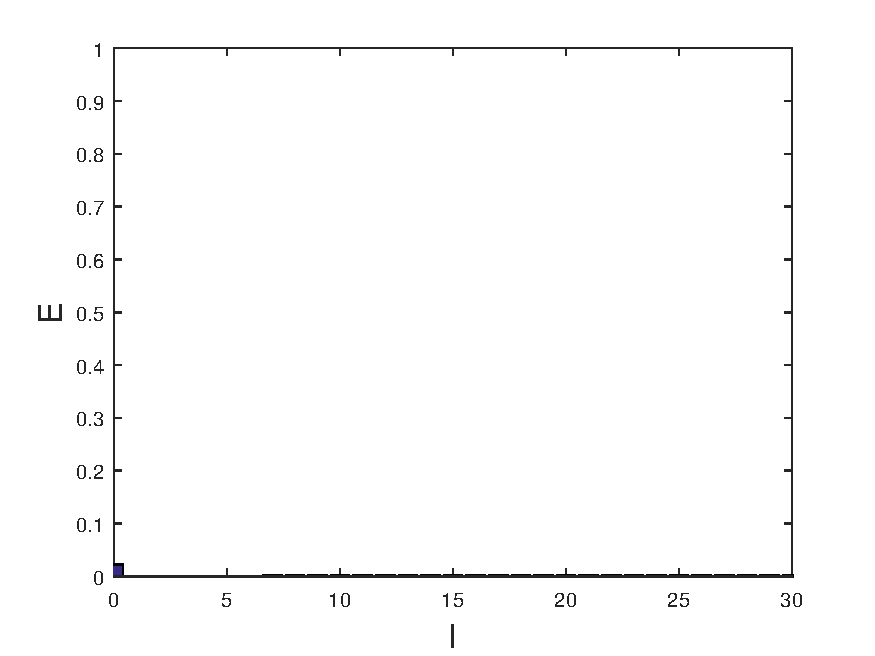
\includegraphics[width=0.45\textwidth]{kugel/Dkonstant/Kugel1_2.pdf}
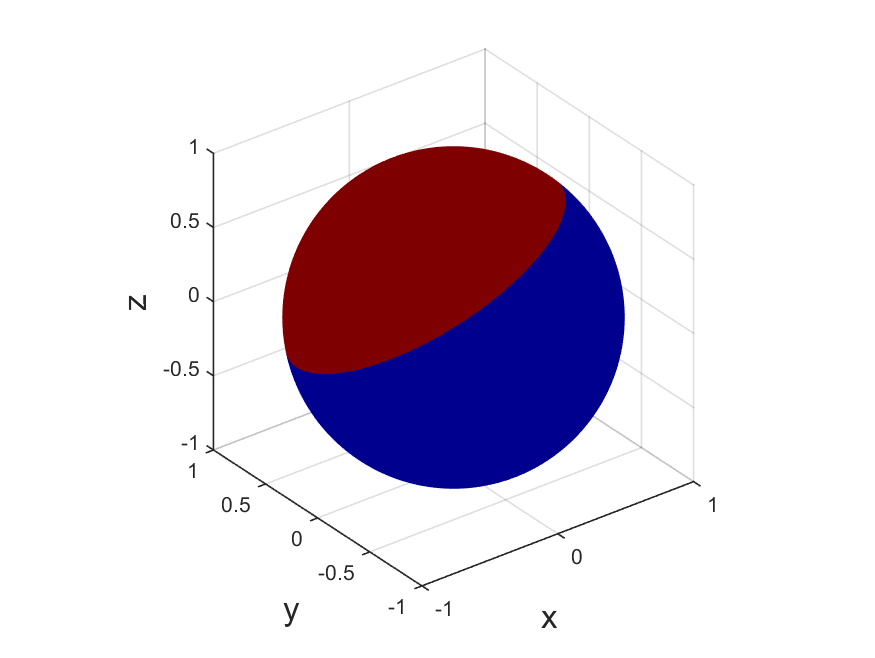
\includegraphics[width=0.45\textwidth]{kugel/Dkonstant/Kugel2_1.pdf}
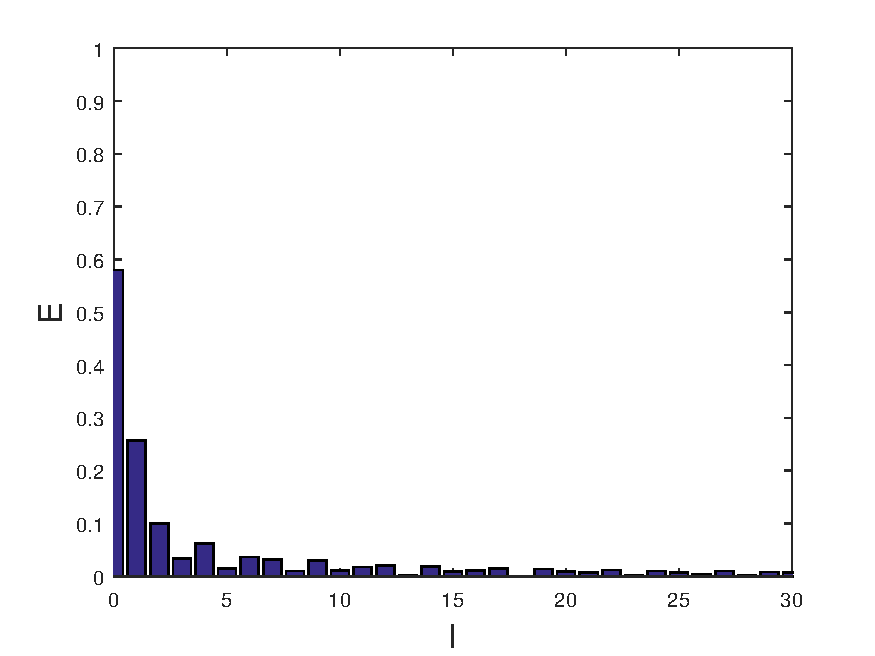
\includegraphics[width=0.45\textwidth]{kugel/Dkonstant/Kugel2_2.pdf}
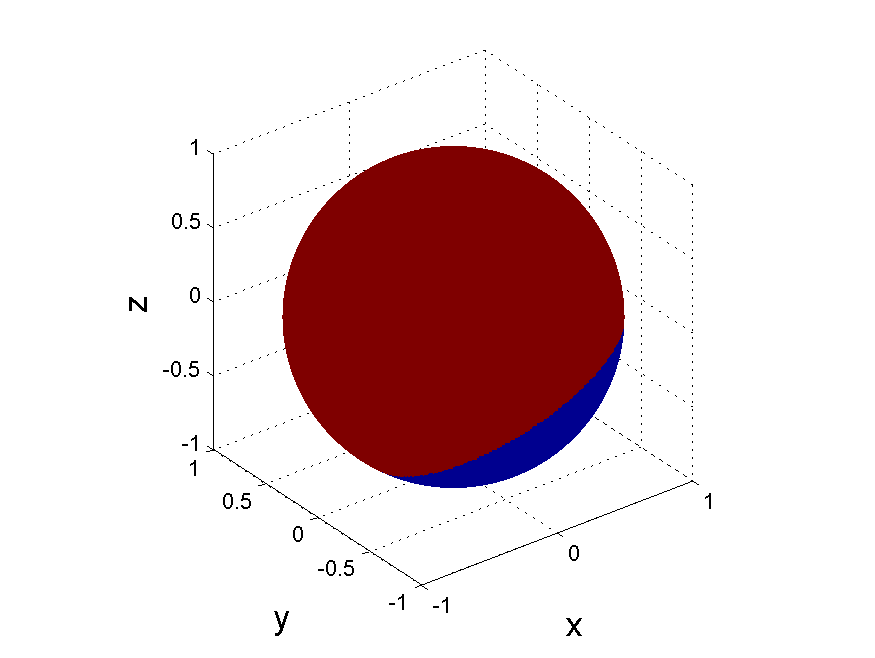
\includegraphics[width=0.45\textwidth]{kugel/Dkonstant/Kugel3_1.pdf}
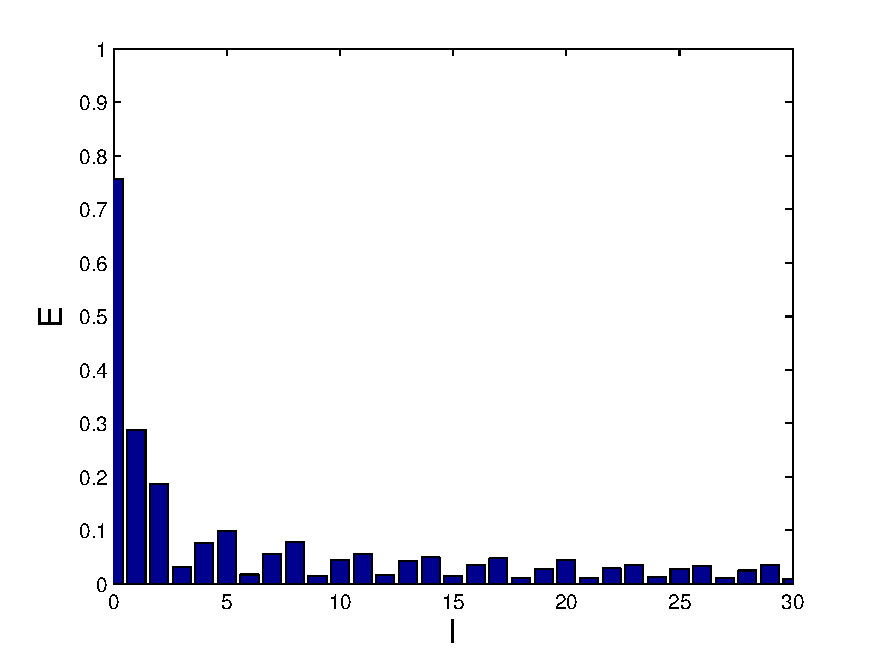
\includegraphics[width=0.45\textwidth]{kugel/Dkonstant/Kugel3_2.pdf}
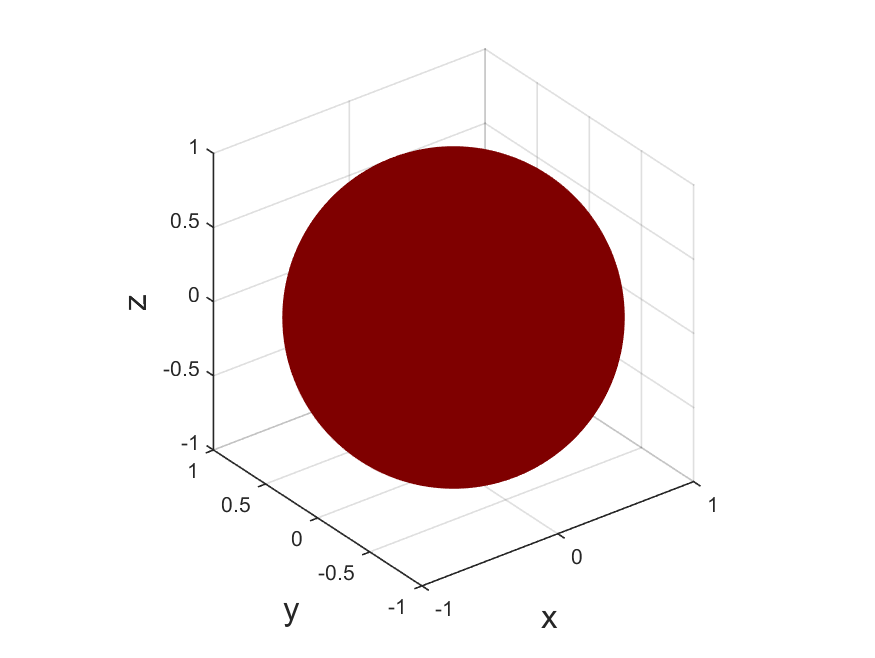
\includegraphics[width=0.45\textwidth]{kugel/Dkonstant/Kugel4_1.pdf}
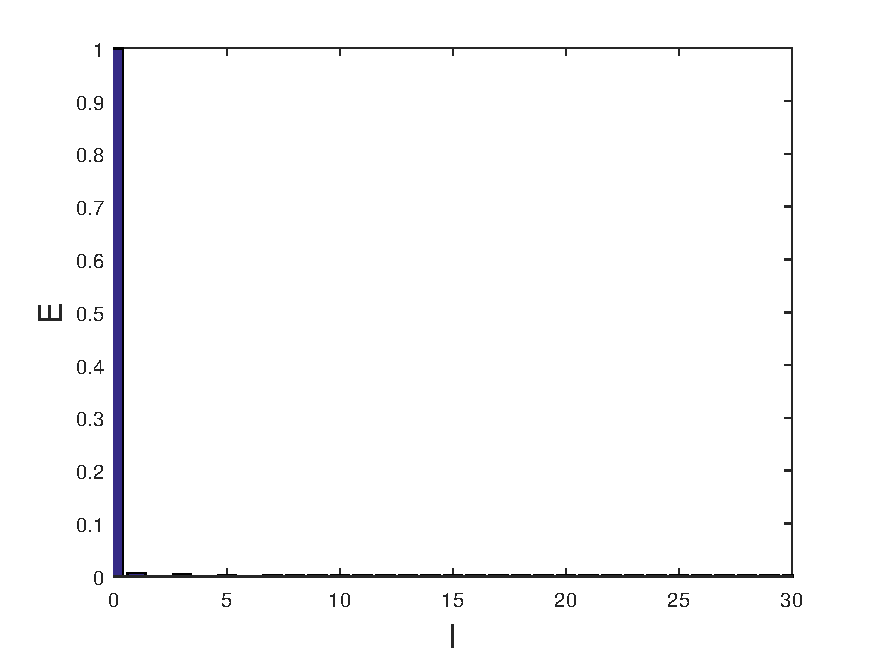
\includegraphics[width=0.45\textwidth]{kugel/Dkonstant/Kugel4_2.pdf}
\caption{Wachsender Kreisabschnitt auf der Kugeloberfl"ache
\label{skript:Dirac2}}
\end{figure}

\section{Gibbs-Ph"anomen}
\rhead{Gibbs-Ph"anomen}
Das Gibbs-Ph"anomen beschreibt, dass man bei der Rekonstruktion einer
Funktion mit Sprungstellen - vor und nach den urspr"unglichen 
Sprungstellen - "Uberschwinger von ca. 9\% der Sprungh"ohe feststellen 
kann sofern die Bandbreite begrenzt wird. 
Bei der Bandbreitenbegrenzung bedeutet, dass nur eine endliche Anzahl 
Fourier-Koeffizienten zur Rekonstruktion einer Funktion verwendet. 
Dieses Ph"anomen m"ochten wir im folgenden Abschnitt f"ur periodische 
Funktionen und Funktionen auf der Kugeloberfl"ache beschreiben und 
illustrieren.

\subsection{Gibbs-Ph"anomen bei einer periodischen Funktion}
In Abbildung \ref{skript:Gibborg} ist die Original-Rechteckfunktion 
dargestellt, von der wir die Fourier-Koeffizienten berechnet haben. 
In Abbildung \ref{skript:Gibbsre} ist die mit den ersten 100 
Fourier-Koeffizienten rekonstruierte Rechteckfunktion zu sehen. 
Es ist deutlich zu erkennen, dass an der Stelle, bei der die 
Original-Rechteckfunktion Sprungstellen aufweist, keine Sprungstellen 
mehr vorhanden sind. 
Stattdessen weist die "Ubergangszone von 0 auf 1 nur noch eine hohe 
Flankensteilheit auf und "uberschwingt kurz vor und nach den 
urspr"unglichen Sprungstellen.
Um auch dies noch besser zu veranschaulichen, ist auf der CD zum Buch 
ein Video zum Gibbs-Ph"anomen bei einer periodischen Funktion.

\subsection{Gibbs-Ph"anomen bei einer Funktion auf der Kugeloberl"ache}
Dasselbe Ph"anomen ist auch bei Funktionen auf der Kugeloberfl"ache 
zu beobachten. 
In den Abbildungen \ref{skript:Gibbs1} und \ref{skript:Gibbs2} sieht 
man die Originalfunktion auf der Kugeloberfl"ache, von der wir - 
wie bei Rechteckfunktion - die Fourier-Koeffizienten berechnet haben. 
In derselben Abbildung sieht man die rekonstruierten Funktionen auf 
der Kugeloberfl"ache. 
Mit dem Parameter $n$ wird jeweils angegeben wie viele 
Fourier-Koeffizienten f"ur die Rekonstruktion der Funktionen 
verwendet wurden. 
Hier ist gut zu erkennen, dass die "Ubergangszone zwischen 0 und 1 
immer schmaler wird, je mehr Fourier-Koeffizienten f"ur die 
Rekonstruktion verwendet wurden. 
Ausserdem sind die "Uberschwinger vor und nach der urspr"unglichen 
Sprungstelle gut zu erkennen.
Um auch dies noch besser zu veranschaulichen, ist auf der CD zum Buch 
ein Video zum Gibbs-Ph"anomen bei einer Funktion auf der Kugeloberl"ache.

\begin{figure}
\begin{minipage}[hbt]{0.5\textwidth}
\centering
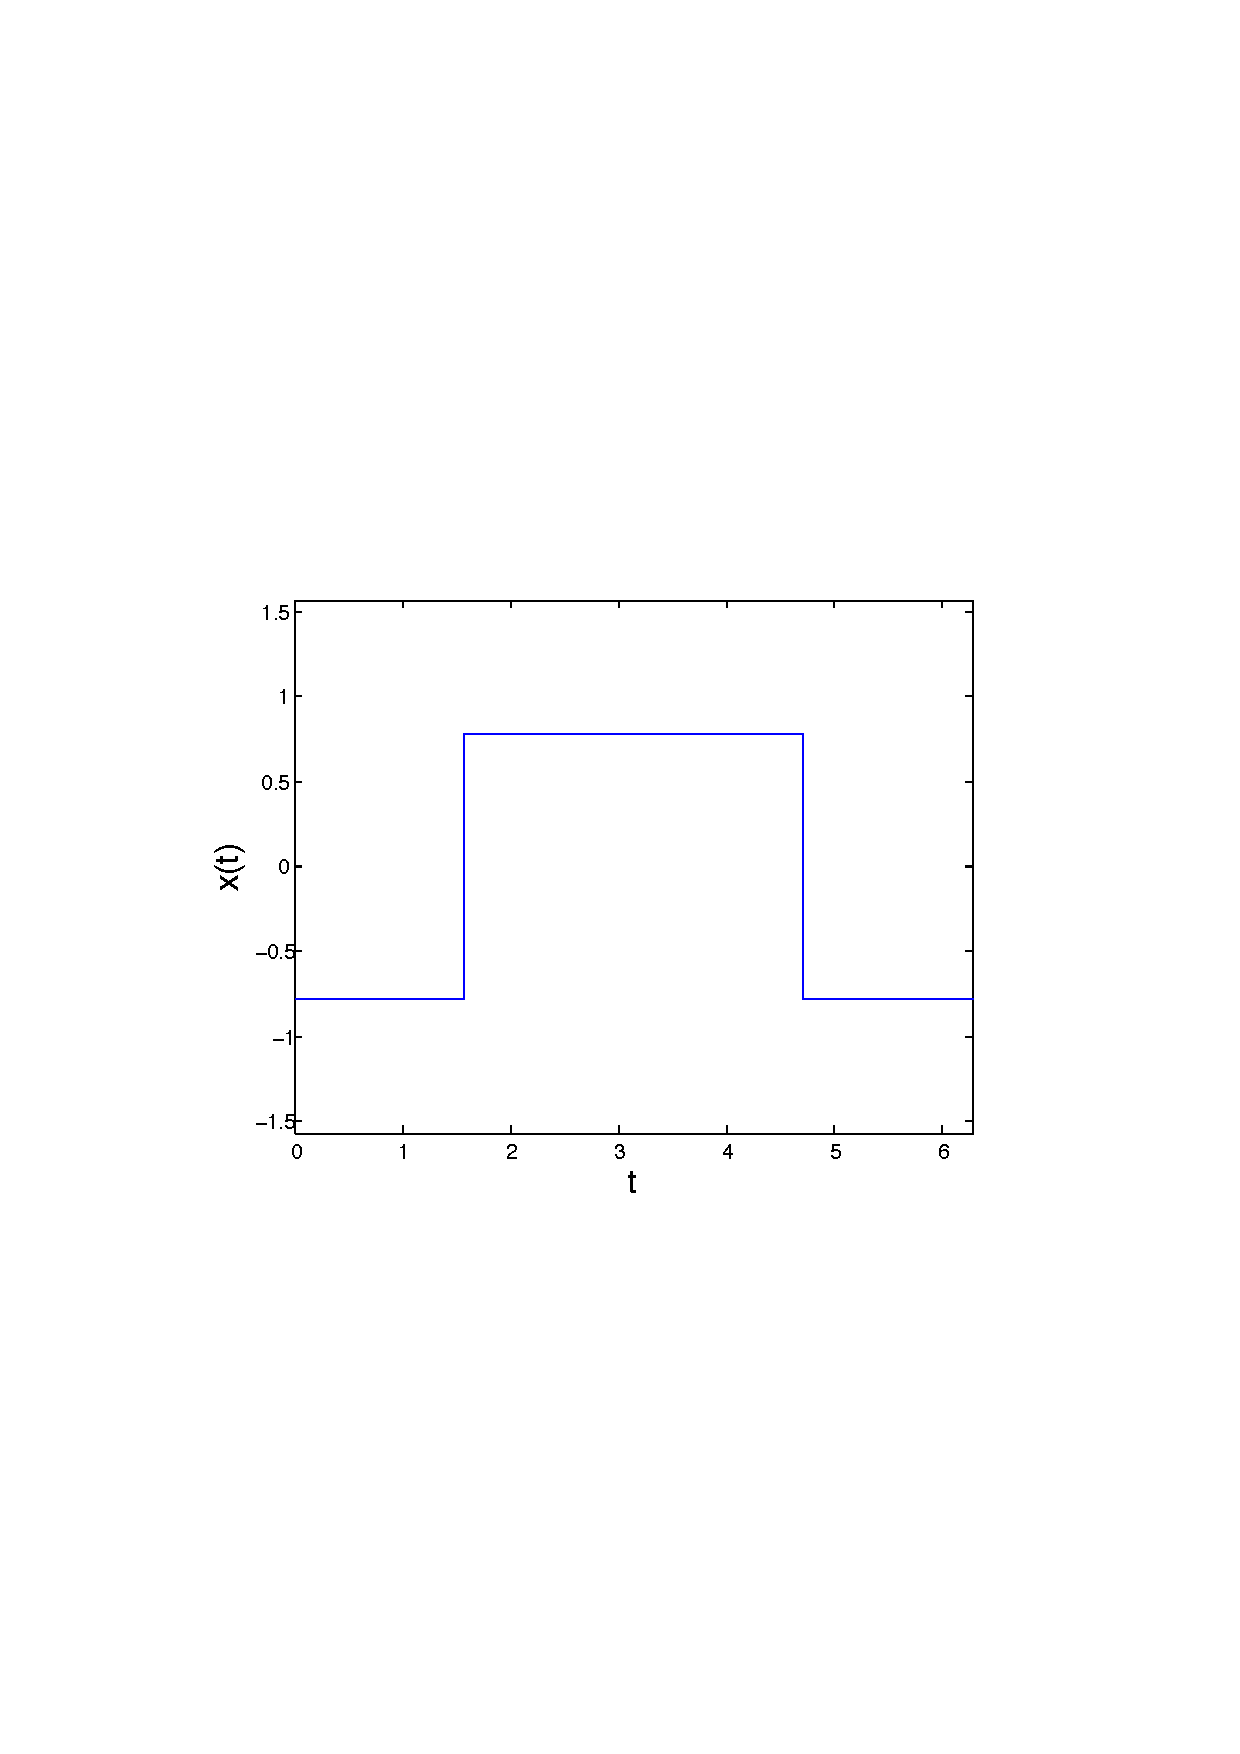
\includegraphics[width=1\textwidth]{kugel/Gibbs/Funktion.pdf}
\caption{Original-Rechteckfunktion}
\label{skript:Gibborg}
\end{minipage}
\hfill
\begin{minipage}[hbt]{0.5\textwidth}
\centering
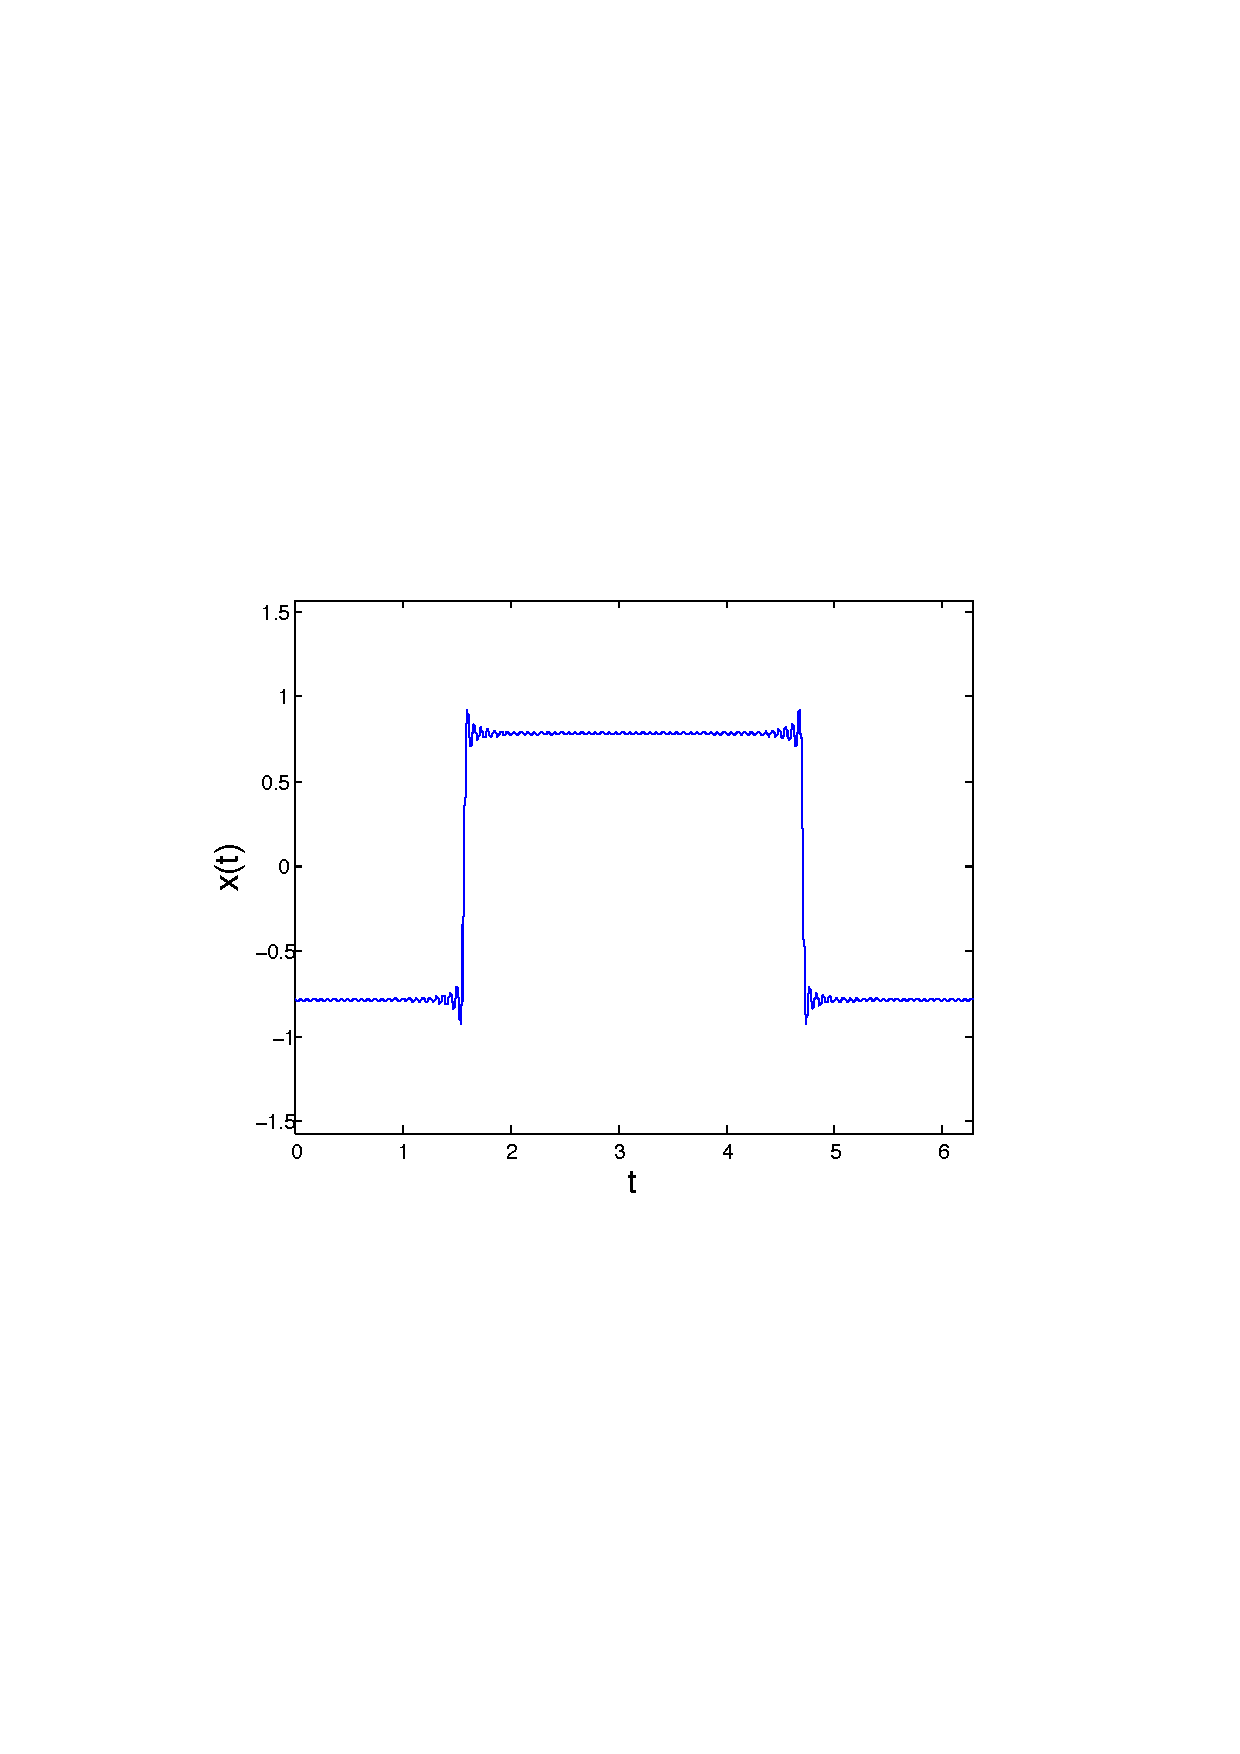
\includegraphics[width=1\textwidth]{kugel/Gibbs/Gibbs.pdf}
\caption{Rekonstruiertes Rechtecksignal}
\label{skript:Gibbsre}
\end{minipage}
\end{figure}

\begin{figure}% Gibbsscher-Effekt
\centering
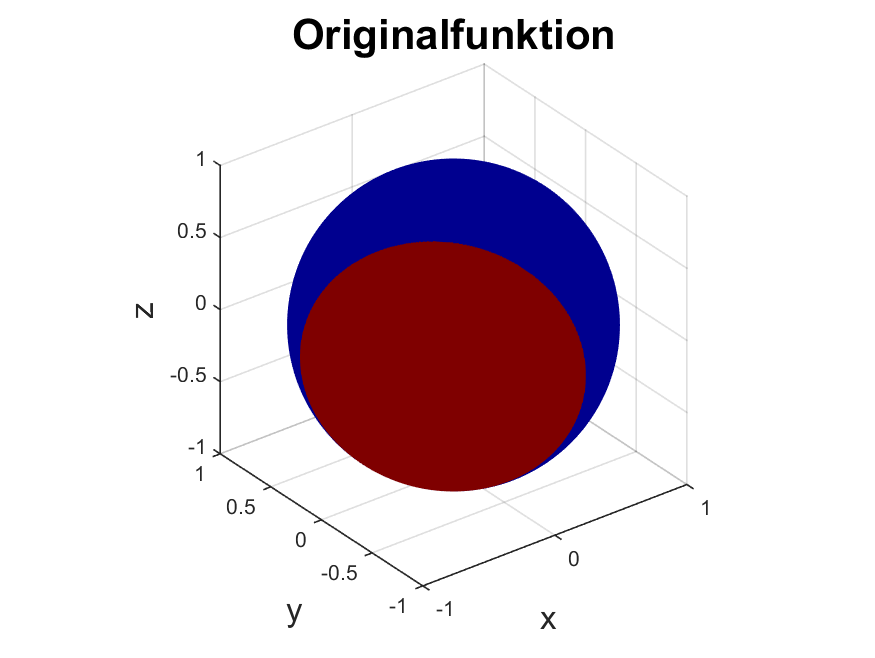
\includegraphics[width=0.4\textwidth]{kugel/Gibbs/GibbsOriginalFunktion.pdf}
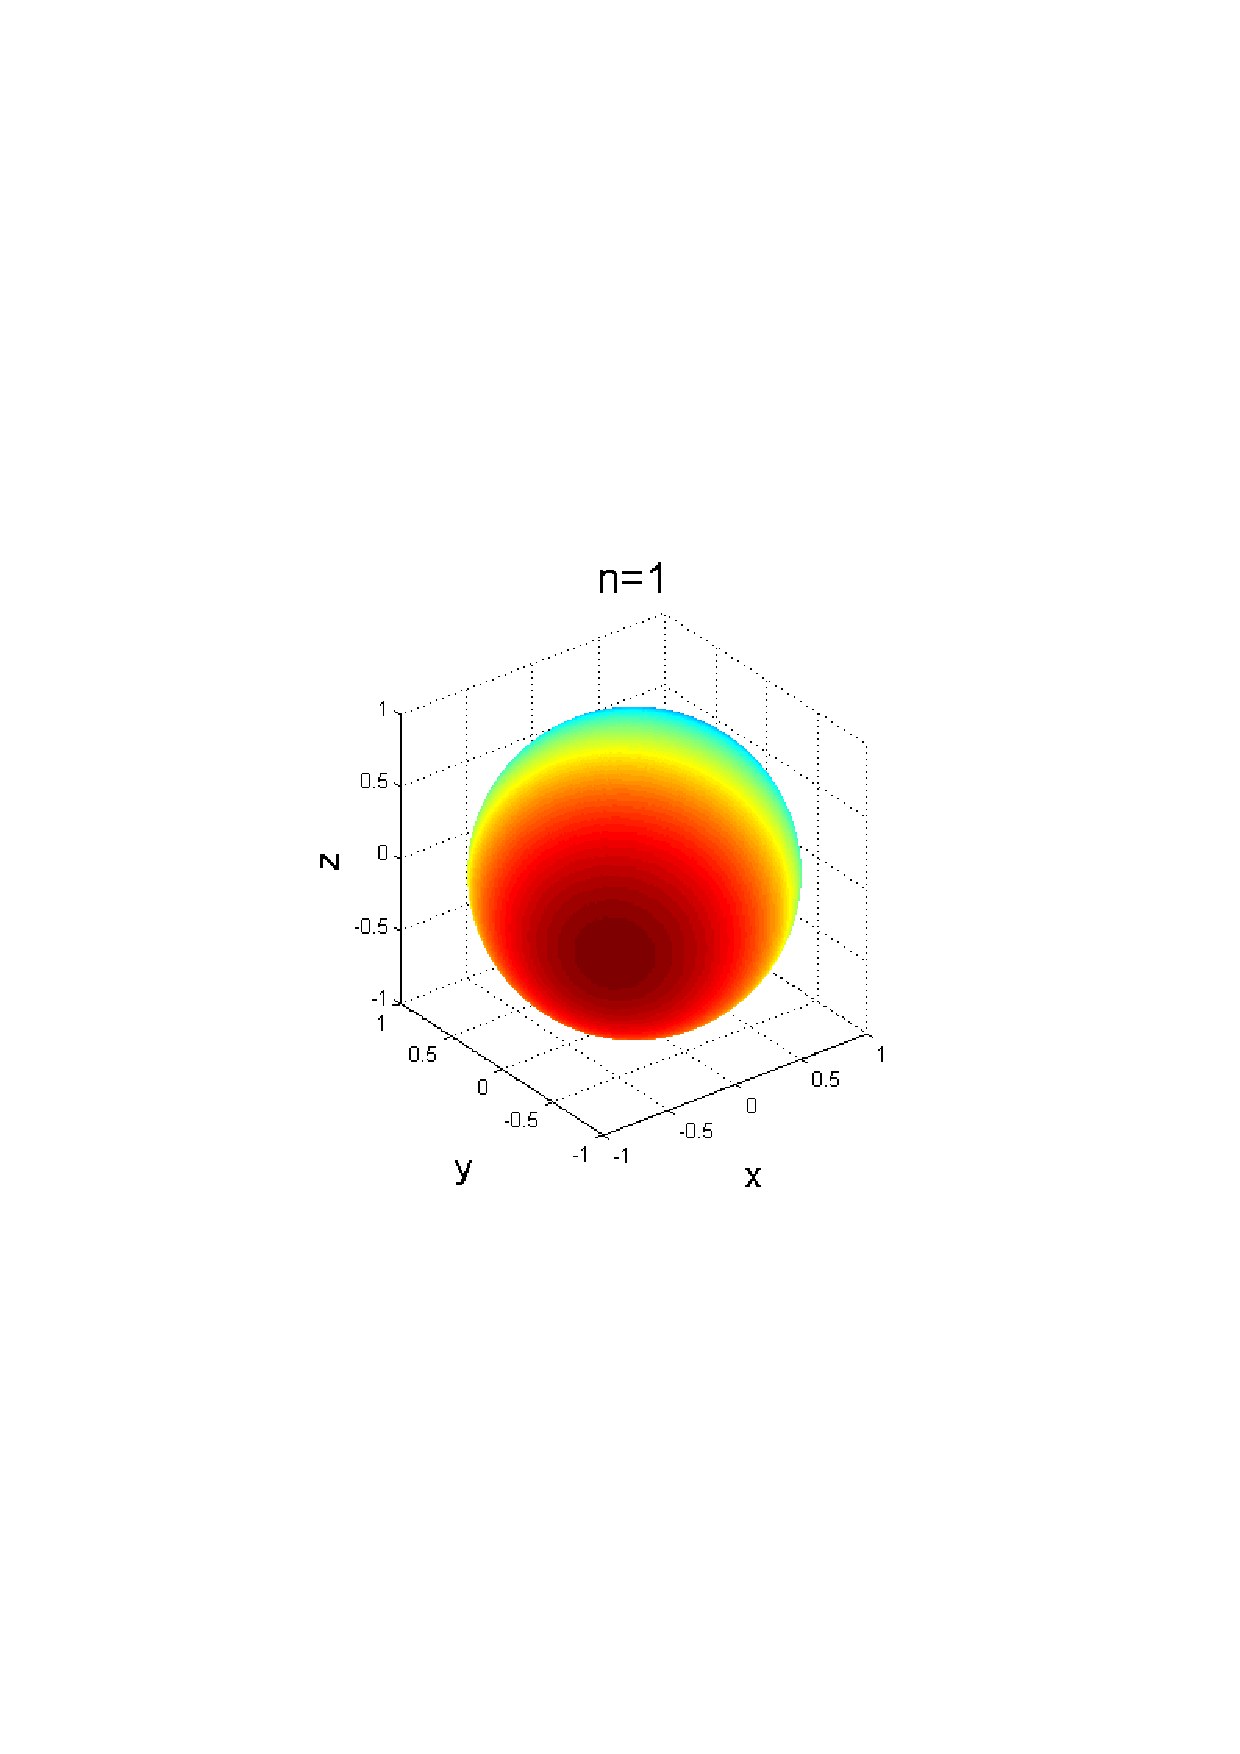
\includegraphics[width=0.4\textwidth]{kugel/Gibbs/GibbsN_1.pdf}
\includegraphics[width=0.4\textwidth]{kugel/Gibbs/GibbsN_2.pdf}
\includegraphics[width=0.4\textwidth]{kugel/Gibbs/GibbsN_3.pdf}
\includegraphics[width=0.4\textwidth]{kugel/Gibbs/GibbsN_4.pdf}
\includegraphics[width=0.4\textwidth]{kugel/Gibbs/GibbsN_5.pdf}
\caption{Gibbs-Ph"anomen mit $n=1$ bis $n=5$
\label{skript:Gibbs1}}
\end{figure}

\begin{figure}% Gibbsscher-Effekt
\centering22
\includegraphics[width=0.4\textwidth]{kugel/Gibbs/GibbsOriginalFunktion.pdf}
\includegraphics[width=0.4\textwidth]{kugel/Gibbs/GibbsN_10.pdf}
\includegraphics[width=0.4\textwidth]{kugel/Gibbs/GibbsN_15.pdf}
\includegraphics[width=0.4\textwidth]{kugel/Gibbs/GibbsN_20.pdf}
\includegraphics[width=0.4\textwidth]{kugel/Gibbs/GibbsN_25.pdf}
\includegraphics[width=0.4\textwidth]{kugel/Gibbs/GibbsN_30.pdf}
\caption{Gibbs-Ph"anomen mit $n=10$ bis $n=30$
\label{skript:Gibbs2}}
\end{figure}

\printbibliography[heading=subbibliography]
\end{refsection}
